% Copyright 2005-2016 Airbus-EDF-IMACS-Phimeca
% Permission is granted to copy, distribute and/or modify this document
% under the terms of the GNU Free Documentation License, Version 1.2
% or any later version published by the Free Software Foundation;
% with no Invariant Sections, no Front-Cover Texts, and no Back-Cover
% Texts.  A copy of the license is included in the section entitled "GNU
% Free Documentation License".

\extanchor{standardparametricmodels}

\renewcommand{\etapemethodo}{B}
\renewcommand{\nomfichier}{docref_B121_DistributionSelection}
\renewcommand{\titrefiche}{Standard parametric models}

\Header

\MathematicalDescription
{

\underline{\textbf{Objective}} \vspace{2mm}

Parametric models aim to describe probability distributions of a random variable with the aid of a limited number of parameters $\vect{\theta}$. Therefore, in the case of continuous variables (i.e. where all possible values are continuous), this means that the probability density of $\vect{X} = \left( X^1,\ldots,X^{n_X} \right)$ can be expressed as $f_X(\vect{x};\vect{\theta})$. In the case of discrete variables (i.e. those which take only discrete values), their probabilities can be described in the form $\Prob{\vect{X} = \vect{x};\vect{\theta}}$.
\vspace{2mm}

The available distributions of OpenTURNS are listed in this section. We start with continuous distributions.

\begin{itemize}
\item {\bf Arcsine distribution}: $\vect{\theta} = \left(a,b \right)$, with the constraint $a<b$. The probability density function writes:

\begin{equation}
\frac{ 1 }{ \pi\frac{b-a}{2} \sqrt{1-\left(\frac{
x-\frac{a+b}{2} }{\frac{b-a}{2} }\right)^{2}} }
\end{equation}
The support is $[a,b]$.

\begin{center}
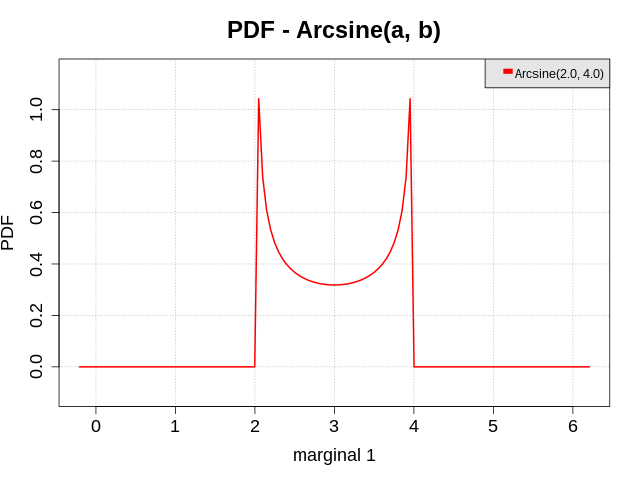
\includegraphics[width=7cm]{Figures/pdf_Arcsine.png}
\end{center}

\item {\bf Beta distribution}: Univariate distribution. $\vect{\theta} = \left( r,t,a,b \right)$, with the constraints $r>0$, $t>r$, $b>a$. The probability density function writes:
\begin{equation}
f_X(x;\vect{\theta}) = \frac{(x-a)^{r-1} (b-x)^{t-r-1}}{(b-a)^{t-1} B(r,t-r)} \mathbf{1}_{a \leq x \leq b}
\end{equation}
where $B$ denotes the Beta function. The support is $[a,b]$.\\
Note that the Epanechnikov distribution is a particular Beta distribution : $Beta (a=-1, b=1, r=2, t=4)$. It is usefull within the kernel smoothing theory (see \otref{docref_B11_KernelSmoothing}{kernel smoothing}).


\begin{figure}[H]
\begin{minipage}{8cm}
\begin{center}
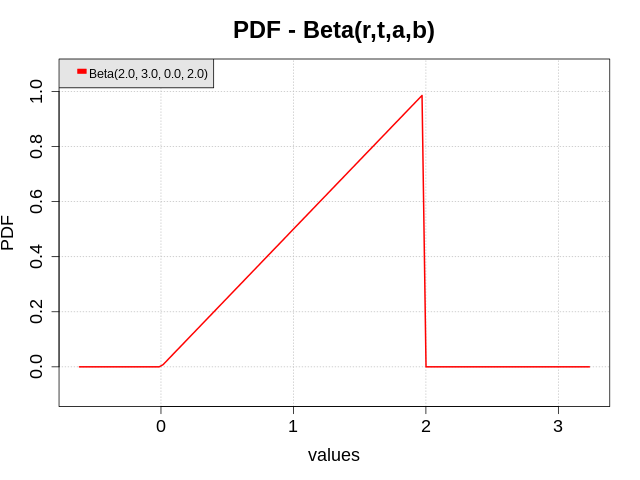
\includegraphics[width=7cm]{Figures/pdf_Beta_1.png}
\caption{PDF of a Beta distribution.}
\end{center}
\end{minipage}
\hfill
\begin{minipage}{8cm}
\begin{center}
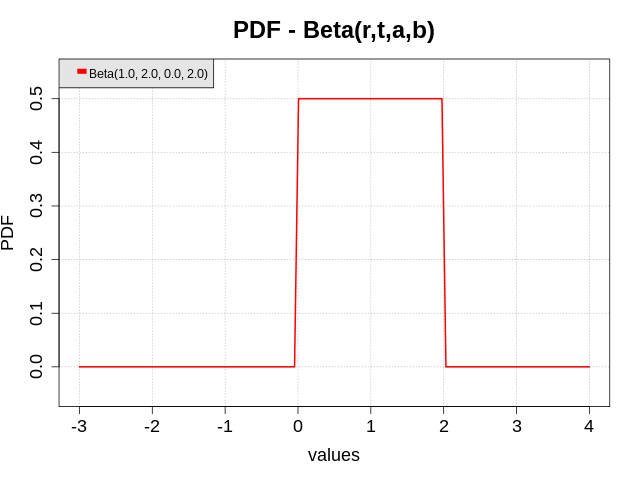
\includegraphics[width=7cm]{Figures/pdf_Beta_2.png}
\caption{PDF of a Beta distribution.}
\end{center}
\end{minipage}
\end{figure}

\begin{figure}[H]
\begin{minipage}{8cm}
\begin{center}
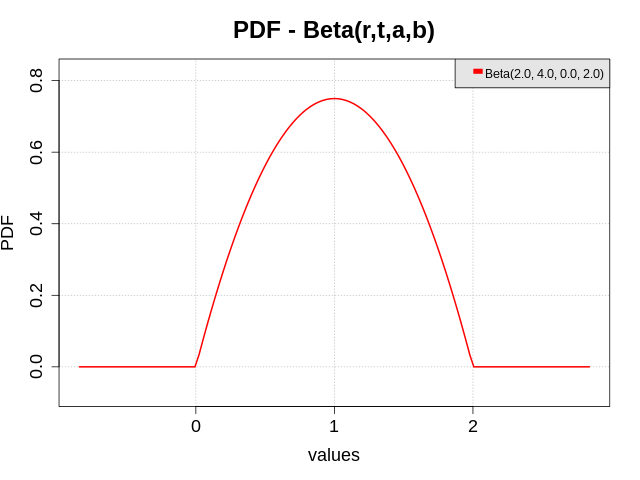
\includegraphics[width=7cm]{Figures/pdf_Beta_3.png}
\caption{PDF of a Beta distribution.}
% \label{PDF3}
\end{center}
\end{minipage}
\hfill
\begin{minipage}{8cm}
\begin{center}
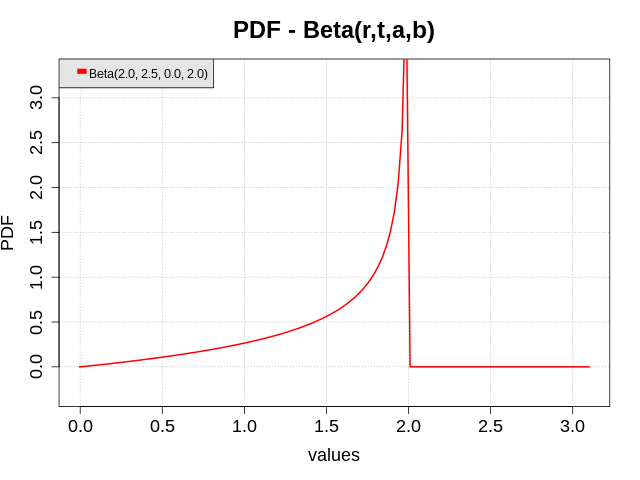
\includegraphics[width=7cm]{Figures/pdf_Beta_4.png}
\caption{PDF of a Beta distribution.}
% \label{PDF4}
\end{center}
\end{minipage}
\end{figure}


\begin{figure}[H]
\begin{minipage}{8cm}
\begin{center}
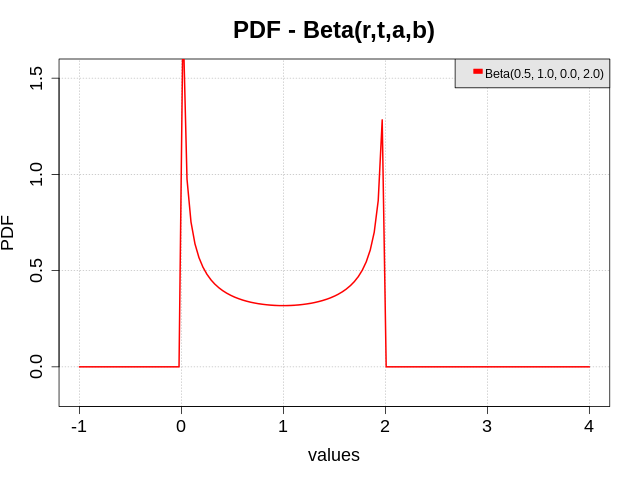
\includegraphics[width=7cm]{Figures/pdf_Beta_5.png}
\caption{PDF of a Beta distribution.}
% \label{PDF5}
\end{center}
\end{minipage}
\hfill
\begin{minipage}{8cm}
\begin{center}
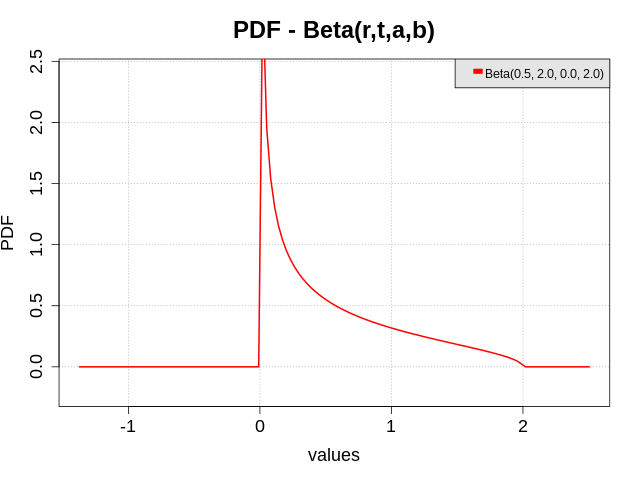
\includegraphics[width=7cm]{Figures/pdf_Beta_6.png}
\caption{PDF of a Beta distribution.}
% \label{PDF6}
\end{center}
\end{minipage}
\end{figure}



\begin{figure}[H]
\begin{minipage}{8cm}
\begin{center}
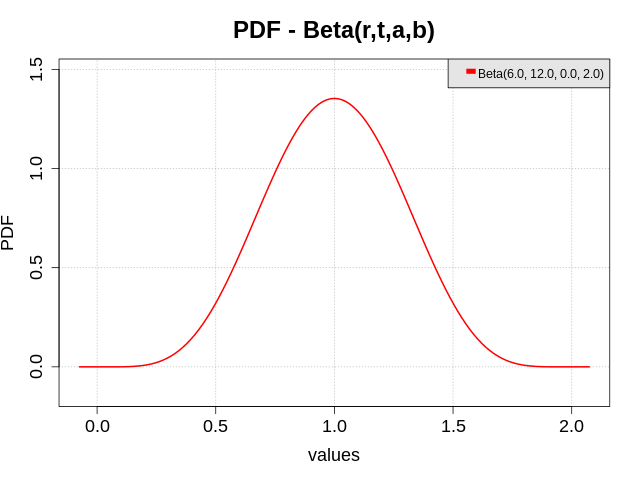
\includegraphics[width=7cm]{Figures/pdf_Beta_7.png}
\caption{PDF of a Beta distribution.}
% \label{PDF7}
\end{center}
\end{minipage}
\hfill
\begin{minipage}{8cm}
\begin{center}
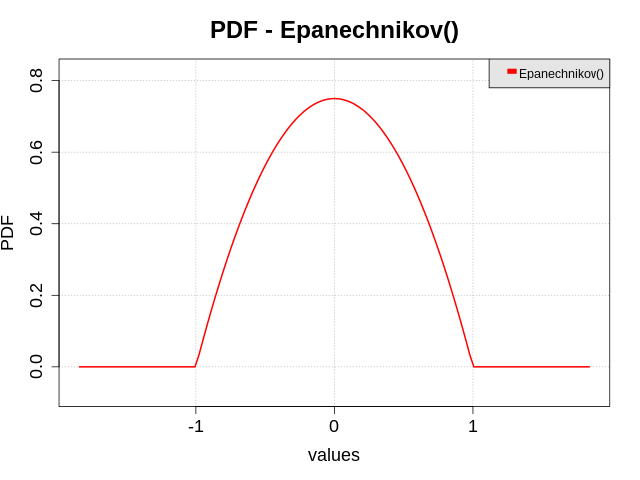
\includegraphics[width=7cm]{Figures/pdf_Epanechnikov.png}
\caption{PDF of a Epanechnikov distribution.}
\label{EpanechnikovPDF}
\end{center}
\end{minipage}
\end{figure}


\item {\bf Burr distribution}: Univariate distribution. $\vect{\theta} = \left( c,k \right)$, with the constraints $c>0$, $k>0$. The probability density function writes:
\begin{equation}
f_X(x;\vect{\theta}) = ck\frac{x^{(c-1)}}{(1+x^c)^{(k+1)}} \mathbf{1}_{x >0}
\end{equation}

\begin{figure}[H]
\begin{minipage}{8cm}
\begin{center}
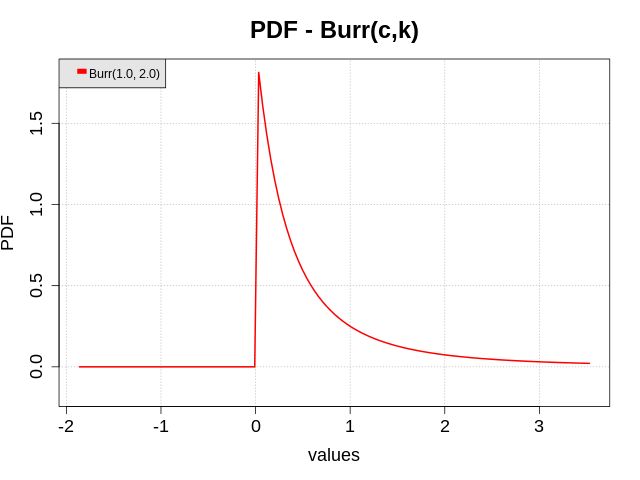
\includegraphics[width=7cm]{Figures/pdf_Burr_1.png}
\caption{PDF of a Burr distribution.}
% \label{PDF30}
\end{center}
\end{minipage}
\hfill
\begin{minipage}{8cm}
\begin{center}
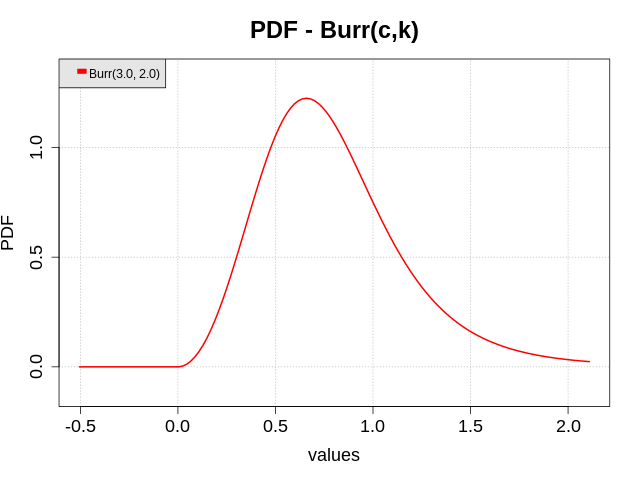
\includegraphics[width=7cm]{Figures/pdf_Burr_2.png}
\caption{PDF of a Burr distribution.}
% \label{PDF31}
\end{center}
\end{minipage}
\end{figure}


\item {\bf Chi}: Univariate distribution. $\vect{\theta} = \nu$ with the constraint $\nu >0$. The probability density function writes:
\begin{equation}
f_X(x;\vect{\theta}) = \displaystyle x^{\nu-1}e^{-x^2/2}\frac{2^{1-\nu^{\strut}/2}}{\Gamma(\nu/2)_{\strut}} \boldsymbol{1}_{[0,+\infty[}(x)
\end{equation}



\begin{figure}[H]
\begin{center}
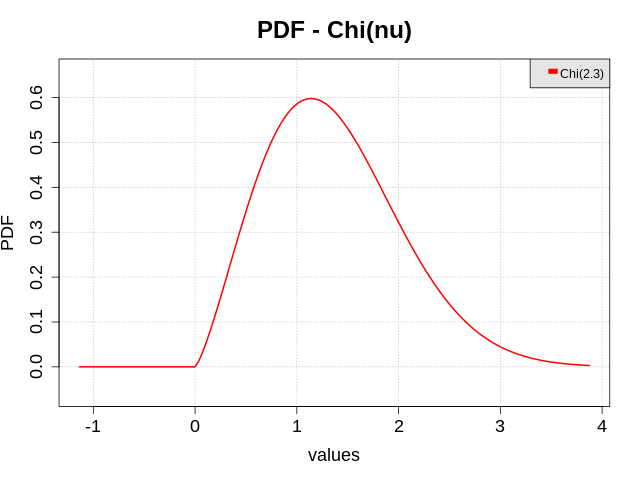
\includegraphics[width=7cm]{Figures/pdf_Chi_1.png}
\caption{PDF of a Chi  distribution.}
% \label{PDF11}
\end{center}
\end{figure}



\item {\bf ChiSquare}: Univariate distribution. $\vect{\theta} = \nu$ with the constraint $\nu >0$. The probability density function writes:
\begin{equation}
f_X(x;\vect{\theta}) = \displaystyle \frac{2^{-\nu^{\strut}/2}}{\Gamma(\nu/2)_{\strut}} x^{(\nu/2-1)}e^{-x/2}\boldsymbol{1}_{[0,+\infty[}(x)
\end{equation}
The support is $[0,+\infty[$.


\begin{figure}[H]
\begin{minipage}{8cm}
\begin{center}
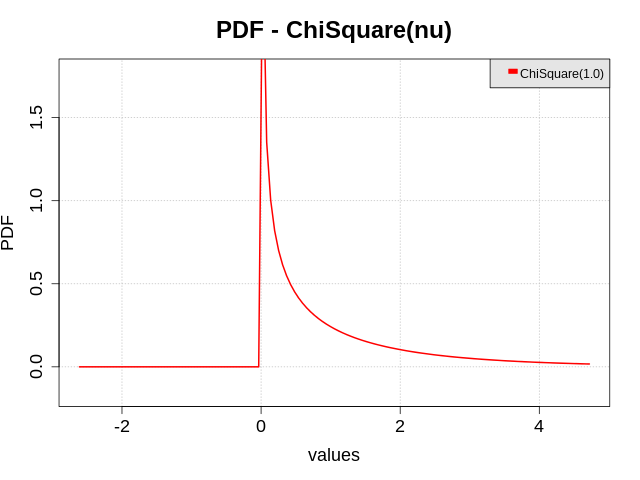
\includegraphics[width=7cm]{Figures/pdf_ChiSquare_1.png}
\caption{PDF of a Chi Square distribution.}
% \label{PDF9}
\end{center}
\end{minipage}
\hfill
\begin{minipage}{8cm}
\begin{center}
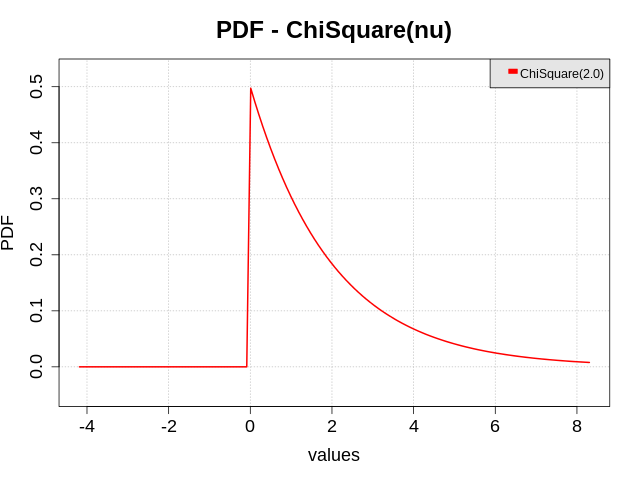
\includegraphics[width=7cm]{Figures/pdf_ChiSquare_2.png}
\caption{PDF of a Chi Square distribution.}
% \label{PDF10}
\end{center}
\end{minipage}
\end{figure}

\begin{figure}[H]
\begin{center}
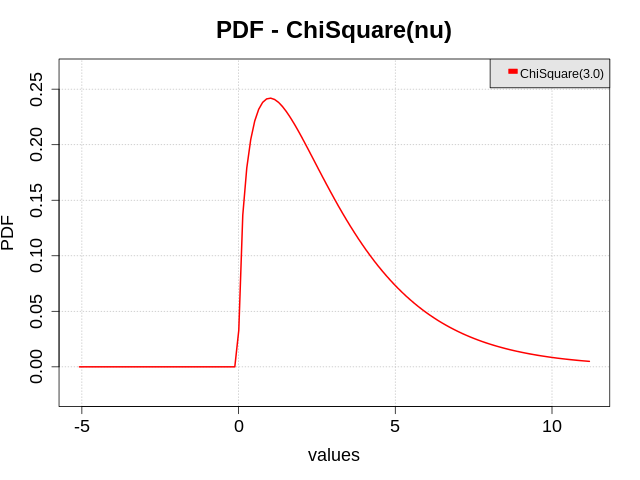
\includegraphics[width=7cm]{Figures/pdf_ChiSquare_3.png}
\caption{PDF of a Chi Square distribution.}
% \label{PDF11}
\end{center}
\end{figure}


\item {\bf Dirichlet distribution}: Multivariate $d$-dimensional distribution. $\vect{\theta} = ( \theta_1, \hdots, \theta_{d+1})$, with the constraints $d \geq 1$ and $\theta_i>0$. The probability density function writes:
\begin{equation}
f_X(\vect{x};\vect{\theta}) = \displaystyle \frac{\Gamma(\sum_{j=1}^{d+1}\theta_j)}{\prod_{j=1}^{d+1}\Gamma(\theta_j)} \left[ 1-\sum_{j=1}^{d} x_j\right]^{(\theta_{d+1}-1)}\prod_{j=1}^d x_j^{(\theta_j-1)}\mathbf{1}_{\Delta}(\vect{x})
\end{equation}
with $\Delta = \{ \vect{x} \in \Rset^d / \forall i, x_i \geq 0, \sum_{i=1}^{d} x_i \leq 1 \}$.



\item {\bf Epanechnikov distribution}: Univariate distribution. The Epanechnikov distribution is a particular Beta distribution : $Beta (a=-1, b=1, r=2, t=4)$. It is usefull within the kernel smoothing theory (see \otref{docref_B11_KernelSmoothing}{kernel smoothing}). See Figure \ref{EpanechnikovPDF} for the graph of its pdf.


\item {\bf Exponential distribution}: $\vect{\theta} = \left( \lambda, \gamma \right)$, with the constraint $\lambda>0$. The probability density function writes:
\begin{equation}
f_X(x;\vect{\theta}) = \lambda \exp \left( -\lambda(x-\gamma) \right) \mathbf{1}_{\gamma \leq x}
\end{equation}
The support is $[\gamma,+\infty[$, and is right skewed. The expected value of the distribution is $\gamma + 1/\lambda$. The coefficient of variation (standard deviation / mean) is equal to $\frac{1}{1+\gamma\lambda}$ and does not depend on $\lambda$ if $\gamma=0$.


\begin{figure}[H]
\begin{center}
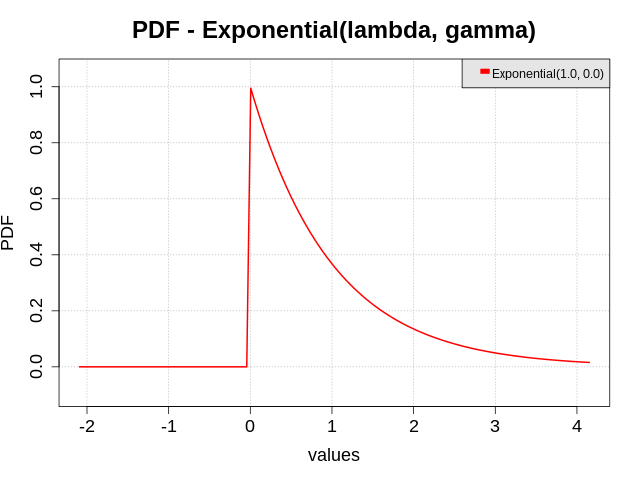
\includegraphics[width=7cm]{Figures/pdf_Exponential.png}
\caption{PDF of an Exponential distribution.}
% \label{PDF12}
\end{center}
\end{figure}


\item {\bf Fisher-Snedecor distribution}: $\vect{\theta} = \left(d_1, d_2 \right)$, with the constraint $d_i>0$. The probability density function writes:
\begin{equation}
f_X(x;\vect{\theta}) = \displaystyle \frac{1}{xB(d_1/2, d_2/2)}\left[\left(\frac{d_1x}{d_1x+d_2}\right)^{d_1/2} \left(1-\frac{d_1x}{d_1x+d_2}\right)^{d_2/2} \right]\mathbf{1}_{x \geq 0}
\end{equation}
The support is $[0,+\infty[$, and is right skewed.

\begin{figure}[H]
\begin{minipage}{8cm}
\begin{center}
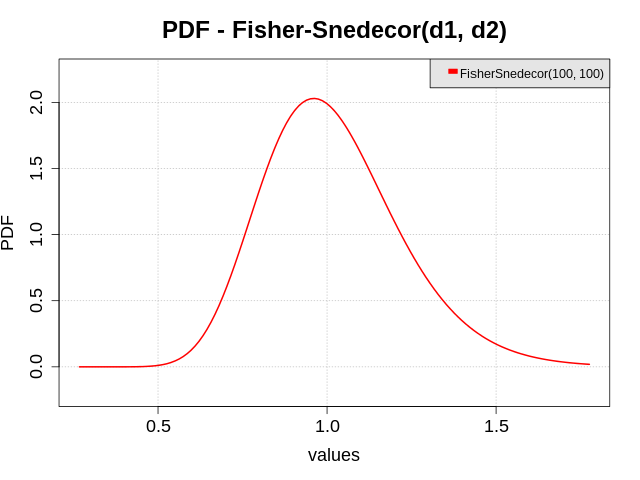
\includegraphics[width=7cm]{Figures/pdf_FisherSnedecor_1.png}
\caption{PDF of a Fisher-Snedecor distribution.}
% \label{PDF13}
\end{center}
\end{minipage}
\hfill
\begin{minipage}{8cm}
\begin{center}
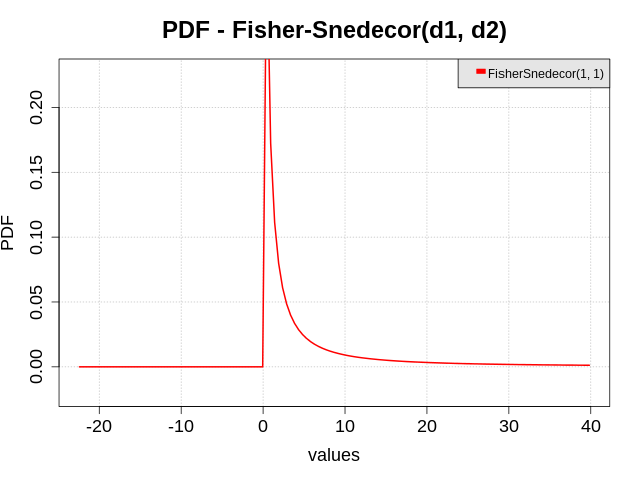
\includegraphics[width=7cm]{Figures/pdf_FisherSnedecor_2.png}
\caption{PDF of a Fisher-Snedecor distribution.}
% \label{PDF14}
\end{center}
\end{minipage}
\end{figure}



\item {\bf Gamma distribution}: Univariate distribution. $\vect{\theta} = \left( \lambda, k, \gamma \right)$, with the constraints  $\lambda>0$, $k>0$. The probability density function writes:
\begin{equation}
f_X(x;\vect{\theta}) = \frac{\lambda}{\Gamma(k)} \left( \lambda(x-\gamma) \right)^{k-1} \exp \left( -\lambda(x-\gamma) \right) \mathbf{1}_{\gamma \leq x}
\end{equation}
where $\Gamma$ is the gamma function. The support is $[\gamma,+\infty[$, and is right skewed.


\begin{figure}[H]
\begin{minipage}{8cm}
\begin{center}
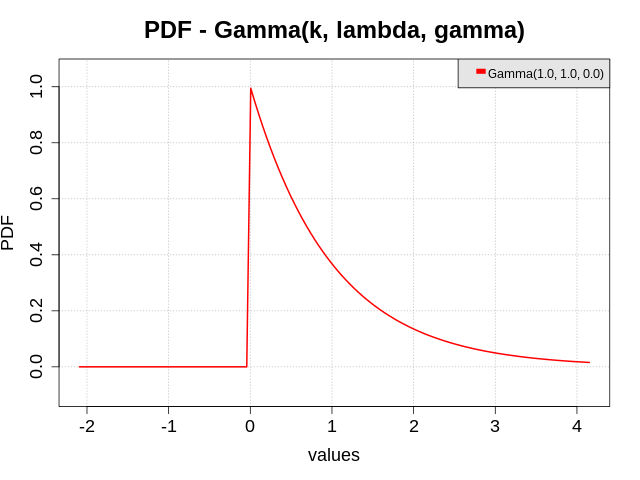
\includegraphics[width=7cm]{Figures/pdf_Gamma_1.png}
\caption{PDF of a Gamma distribution.}
% \label{PDF13}
\end{center}
\end{minipage}
\hfill
\begin{minipage}{8cm}
\begin{center}
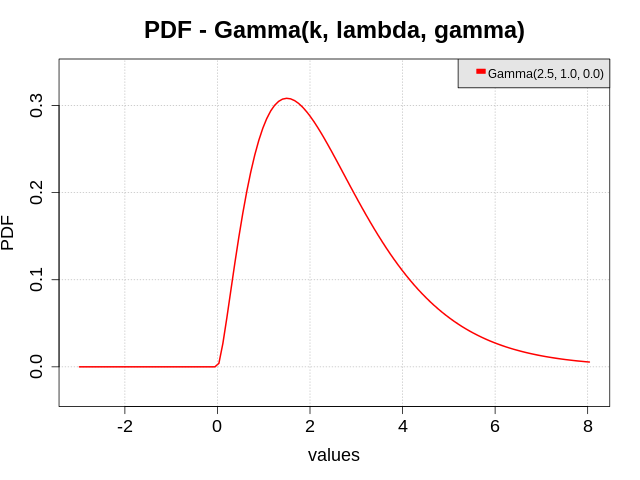
\includegraphics[width=7cm]{Figures/pdf_Gamma_2.png}
\caption{PDF of a Gamma distribution.}
% \label{PDF14}
\end{center}
\end{minipage}
\end{figure}

\begin{figure}[H]
\begin{center}
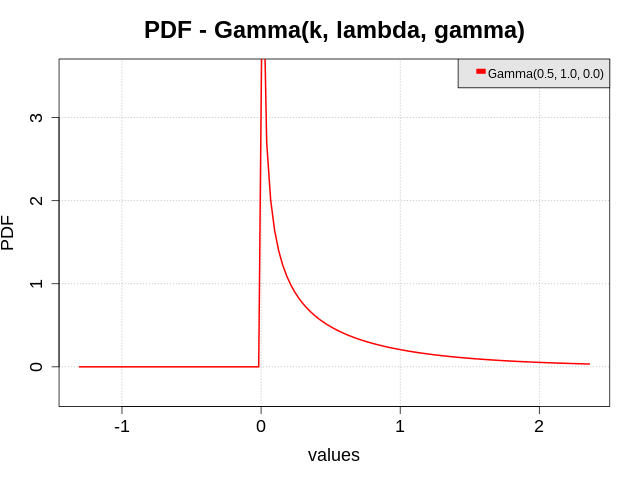
\includegraphics[width=7cm]{Figures/pdf_Gamma_3.png}
\caption{PDF of a Gamma distribution.}
% \label{PDF15}
\end{center}
\end{figure}



\item {\bf Generalized Pareto distribution}: Univariate
distribution. $\vect{\theta} = \left( \xi, \sigma \right)$, with the constraints  $\sigma>0$. The cumulative probability function writes:
\begin{equation}
F_X(x;\vect{\theta}) = \left\{
\begin{array}{ll}
\displaystyle 1-\left(
1+\frac{\xi x}{\sigma}\right)_{\strut}^{-1/\xi} & \mbox{if } \xi \neq 0 \\
\displaystyle 1-\exp\left(-\frac{x}{\sigma}\right) & \mbox{if } \xi = 0
\end{array}
\right.
\end{equation}
The support is $\Rset^+$ if $\xi \geq 0$ and $[0, -\frac{1}{\xi}]$ if $\xi < 0$.

\begin{figure}[H]
\begin{minipage}{8cm}
\begin{center}
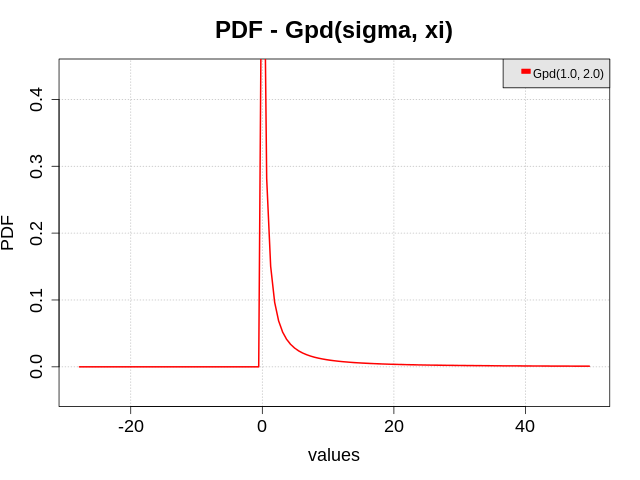
\includegraphics[width=7cm]{Figures/pdf_GPD_1.png}
\caption{PDF of a Generalized Pareto distribution.}
\end{center}
\end{minipage}
\hfill
\begin{minipage}{8cm}
\begin{center}
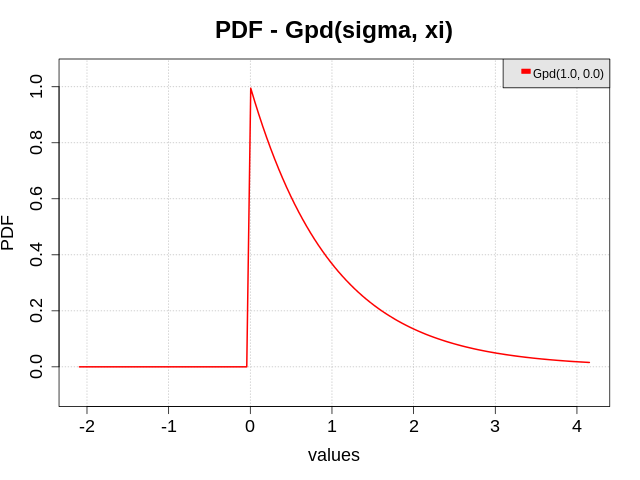
\includegraphics[width=7cm]{Figures/pdf_GPD_2.png}
\caption{PDF of a Generalized Pareto distribution.}
\end{center}
\end{minipage}
\end{figure}


\item {\bf Gumbel distribution}: Univariate distribution. $\vect{\theta} = \left( \alpha,\beta \right)$, with the constraint $\alpha>0$. The probability density function writes:
\begin{equation}
f_X(x;\vect{\theta}) = \alpha \exp \left( -\alpha(x-\beta) - e^{-\alpha(x-\beta)} \right)
\end{equation}

The support is $\Rset$. $\beta$ describes the most likely value, but this is less than the expected value of the distribution because the distribution is asymmetric (right skewed): the probability values in the distribution's right tail (i.e. values greater than $\beta$) decrease more gradually than those in the left tail (i.e. values less than $\beta$). a provides a measure of dispersion: the probability density function flattens as $\alpha$ decreases.

\begin{figure}[H]
\begin{center}
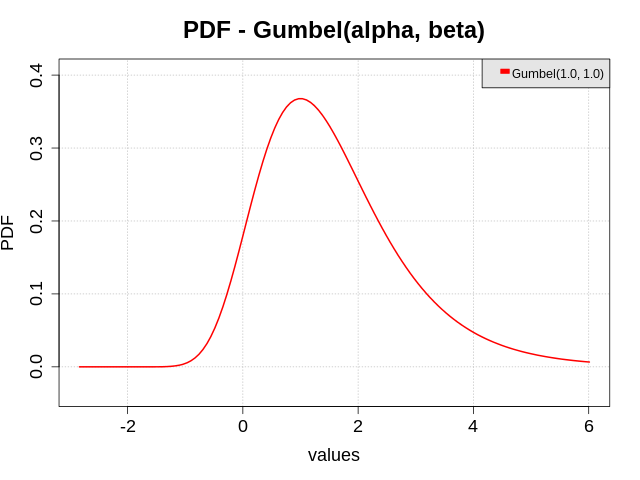
\includegraphics[width=7cm]{Figures/pdf_Gumbel.png}
\caption{PDF of a Gumbel distribution.}
% \label{PDF16}
\end{center}
\end{figure}


\item {\bf Histogram distribution}: Univariate distribution. $\vect{\theta} = \left( (l_i, h_i)_i \right)$, with the constraint $h_i>0$ and $l_i>0$. The probability density function writes:
\begin{equation}
f_X(x;\vect{\theta}) = \sum_{i=1}^{n}H_i\;\boldsymbol{1}_{[x_i,x_{i+1}]}(x)
\end{equation}
where
\begin{itemize}
\item $H_i=h_i/S$ is the normalized heights, with $S=\sum_{i=1}^nh_i\,l_i$ being the initial surface of the histogram.
\item $l_i = x_{i+1} - x_i$, $1\leq i \leq n$
\item $n$ is the size of the HistogramPairCollection
\end{itemize}



\begin{figure}[H]
\begin{minipage}{8cm}
\begin{center}
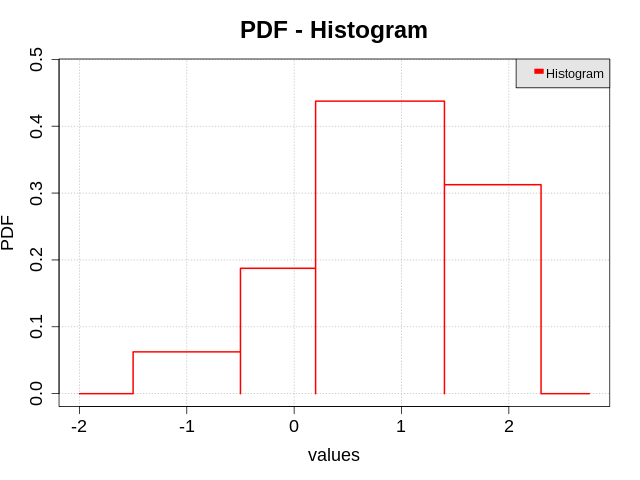
\includegraphics[width=7cm]{Figures/pdf_Histogram.png}
\caption{PDF of a Histogram distribution.}
\end{center}
\end{minipage}
\hfill
\begin{minipage}{8cm}
\begin{center}
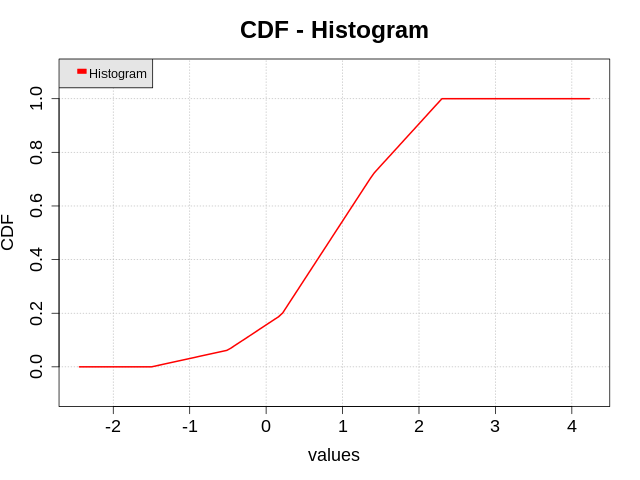
\includegraphics[width=7cm]{Figures/cdf_Histogram.png}
\caption{PDF of a Histogram distribution.}
\end{center}
\end{minipage}
\end{figure}


\item {\bf Inverse ChiSquare distribution}: Univariate distribution.  $\vect{\theta} = \left( \nu \right)$,, with the constraint $\nu>0$. The probability density function writes:
\begin{equation}
f_X(x;\vect{\theta}) = \dfrac{\exp \left( -\frac{1}{2 x}\right)}{\Gamma \left(\frac{\nu}{2}\right)\lambda^{\frac{\nu}{2}}x^{\frac{\nu}{2}+1}} \mathbf{1}_{x>0}
\end{equation}
A Inverse ChiSquare distribution  parametered by $\nu$ is exactly the InverseGamma distribution parametered by $(\dfrac{\nu}{2}, 2)$.

\begin{figure}[H]
\begin{center}
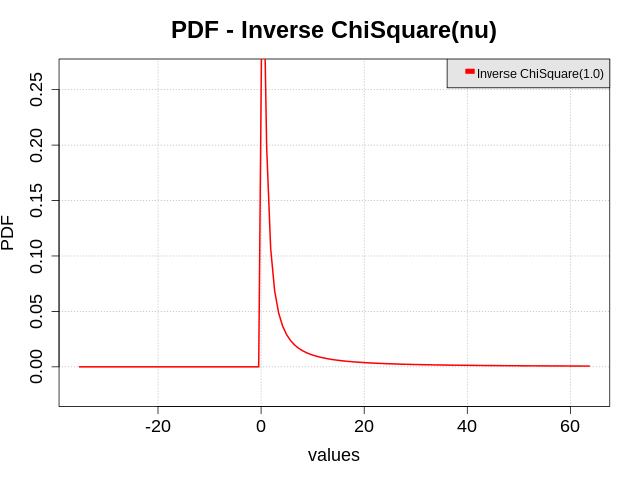
\includegraphics[width=7cm]{Figures/pdf_InverseChiSquare.png}
\caption{PDF of an Inverse ChiSquare distribution.}
% \label{PDFICS}
\end{center}
\end{figure}

\item {\bf Inverse Gamma distribution}: Univariate distribution.  $\vect{\theta} = \left( k, \lambda \right)$,, with the constraint $k>0$ and $\lambda>0$. The probability density function writes:
\begin{equation}
f_X(x;\vect{\theta}) = \displaystyle  \frac{\exp \left( -\dfrac{1}{\lambda x}\right)}{\Gamma^{\strut}(k)\lambda^kx^{k+1}} \mathbf{1}_{x>0}
\end{equation}

\begin{figure}[H]
\begin{center}
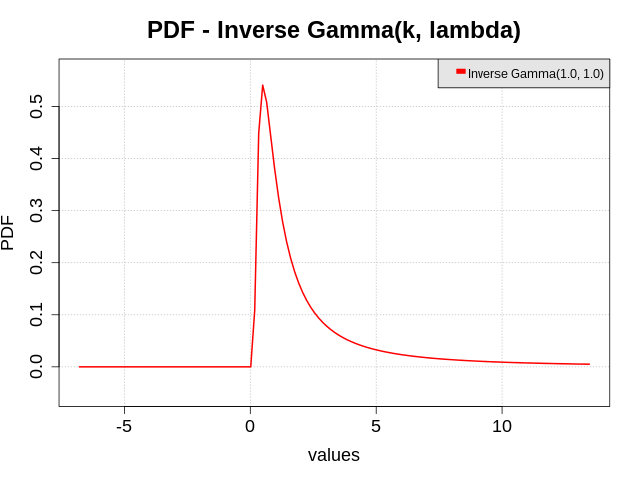
\includegraphics[width=7cm]{Figures/pdf_InverseGamma.png}
\caption{PDF of an Inverse Gamma distribution.}
% \label{PDFIG}
\end{center}
\end{figure}



\item {\bf Inverse Normal distribution}: Univariate distribution. $\vect{\theta} = \left( \lambda,\mu \right)$, with the constraint $\lambda>0$ and $\mu>0$. The probability density function writes:
\begin{equation}
f_X(x;\vect{\theta}) = \displaystyle \left(\frac{\lambda}{2\pi x^3} \right)^{1/2}e^{-\lambda(x-\mu)^2/(2\mu^2x)} \mathbf{1}_{x>0}
\end{equation}


\begin{figure}[H]
\begin{minipage}{8cm}
\begin{center}
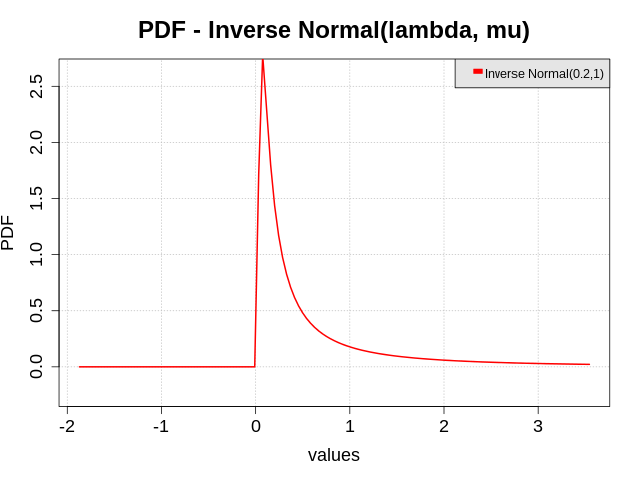
\includegraphics[width=7cm]{Figures/pdf_InverseNormal_1.png}
\caption{PDF of a Inverse Normal distribution.}
% \label{PDF13}
\end{center}
\end{minipage}
\hfill
\begin{minipage}{8cm}
\begin{center}
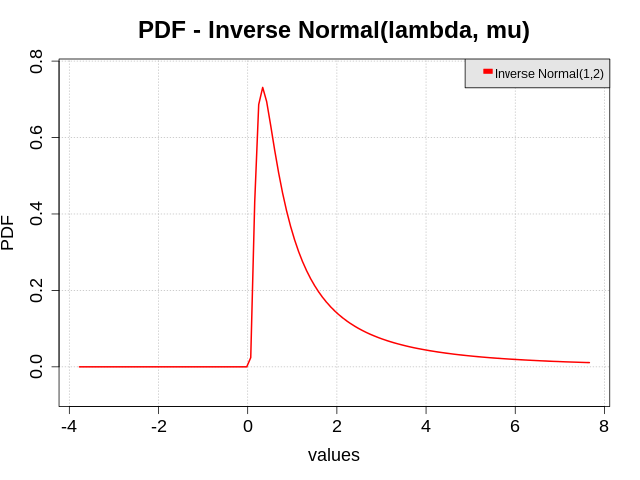
\includegraphics[width=7cm]{Figures/pdf_InverseNormal_2.png}
\caption{PDF of a  Inverse Normal distribution.}
% \label{PDF14}
\end{center}
\end{minipage}
\end{figure}



\item {\bf Inverse Wishart distribution}: Multivariate distribution. $\vect{\theta} = \left( \mat{V},\nu \right)$ where $\mat{V}$ is a symmetric positive definite matrix of dimension $p$ and $\nu>p-1$. The probability density function writes:
\begin{equation}
f_{\vect{x}}(\vect{x};\vect{\theta}) = \frac{|\mat{V}|^{\frac{\nu}{2}}e^{-\frac{\mathrm{tr}(\mat{V}m(\vect{x})^{-1})^{\strut}}{2}}}{2^{\frac{\nu p}{2}}|m(\vect{x})|^{\frac{\nu+p+1}{2}}\Gamma_p\left(\frac{\nu}{2}\right)_{\strut}}\fcar{\cM_p^+(\Rset)}{m(\vect{x})}
\end{equation}
where $\vect{x}\in\Rset^{\frac{p(p+1)}{2}}$, $\cM_p^+(\Rset)$ is the set of symmetric positive matrices of dimension $p$ and $m:\Rset^{\frac{p(p+1)}{2}}\rightarrow\cM_p^+(\Rset)$ is given by:
\begin{align}
  m(\vect{x})=\left(\begin{array}{cccc}
x_1 & x_2 & \cdots &  x_{1+p(p-1)/2}\\
x_2 & x_3 &  & \vdots \\
\vdots & & \ddots & \vdots\\
x_{1+p(p-1)/2} & \cdots & \cdots & x_{p(p+1)/2}
\end{array}
\right)
\end{align}

\item {\bf Laplace distribution}: Univariate distribution. $\vect{\theta} = \left( \lambda, \mu \right)$, with the constraint $\lambda>0$. The probability density function writes:
\begin{equation}
f_X(x;\vect{\theta}) = \displaystyle \frac{\lambda^{\strut}}{2_{\strut}}e^{-\lambda |x-\mu|}
\end{equation}

The Laplace distribution is the generalisation of the Exponential distribution to the range $\Rset$.

\begin{figure}[H]
\begin{center}
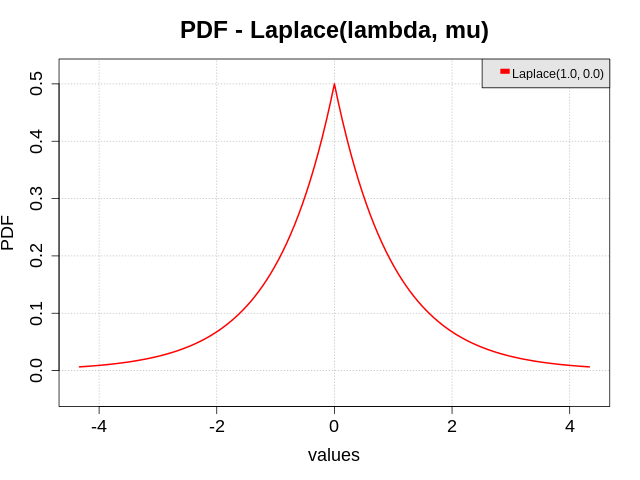
\includegraphics[width=7cm]{Figures/pdf_Laplace.png}
\caption{PDF of a Laplace distribution.}
% \label{PDF17}
\end{center}
\end{figure}





\item {\bf Logistic distribution}: Univariate distribution. $\vect{\theta} = \left(\alpha,\beta \right)$, with the constraint $\beta \geq 0$. The probability density function writes:
\begin{equation}
f_X(x;\vect{\theta}) = \frac{\exp \left( -\frac{x-\alpha}{\beta} \right)}{\beta \left[ 1+\exp \left( -\frac{x-\alpha}{\beta} \right) \right]^2}
\end{equation}
The support is $\Rset$. $\alpha$ describes the most likely value. $\beta$ provides a measure of dispersion: the probability density function flattens as $\beta$ decreases.

\begin{figure}[H]
\begin{center}
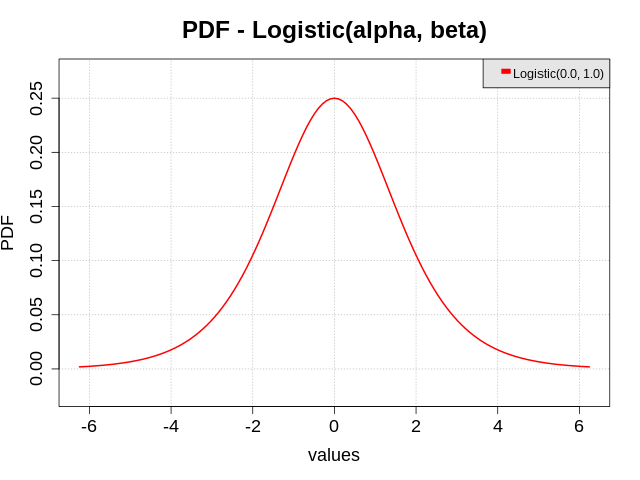
\includegraphics[width=7cm]{Figures/pdf_Logistic.png}
\caption{PDF of a  logistic distribution.}
% \label{PDF18}
\end{center}
\end{figure}


\item {\bf LogNormal distribution}: Univariate distribution. $\vect{\theta} = \left(\mu_\ell,\sigma_\ell,\gamma \right)$, with the constraint $\sigma_\ell>0$. The probability density function writes:
\begin{equation}
f_X(x;\vect{\theta}) = \frac{1}{\sigma_\ell (x-\gamma) \sqrt{2\pi}} \exp \left( -\frac{1}{2} \left( \frac{\textrm{ln}(x-\gamma)-\mu_\ell}{\sigma_\ell}  \right)^2 \right) \mathbf{1}_{\gamma \leq x}
\end{equation}
The support is $[\gamma,+\infty[$, and is right skewed.

\begin{figure}[H]
\begin{center}
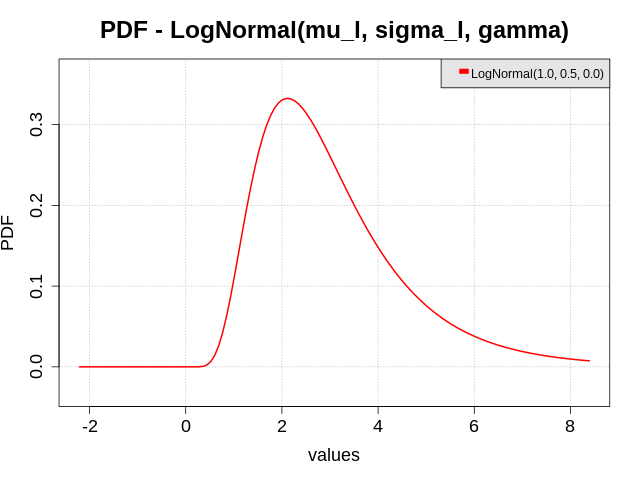
\includegraphics[width=7cm]{Figures/pdf_LogNormal.png}
\caption{PDF of a  LogNormal distribution.}
% \label{PDF19}
\end{center}
\end{figure}


\item {\bf LogUniform distribution}: Univariate distribution. $\vect{\theta} = \left(a_\ell,b_\ell\right)$, with the constraint $b_\ell>a_\ell$. The probability density function writes:
\begin{equation}
f_X(x;\vect{\theta}) = \frac{1}{x(b_\ell-a_\ell)}\mathbf{1}_{a_\ell \leq \log(x) \ leq b_\ell}
\end{equation}
The support is $[\exp(a_\ell),\exp(b_\ell)]$, and is right skewed.

\begin{figure}[H]
\begin{center}
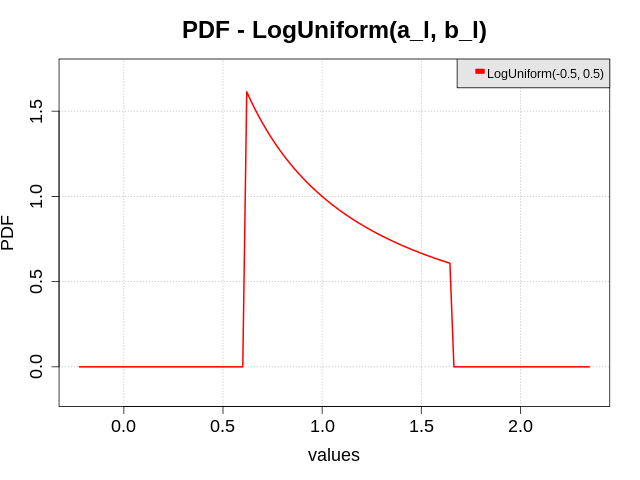
\includegraphics[width=7cm]{Figures/pdf_LogUniform.png}
\caption{PDF of a  LogUniform distribution.}
% \label{PDF19}
\end{center}
\end{figure}

\item {\bf Maximum entropy statistics distribution}: Multivariate distribution, parametrized by $d$ marginals, with bounds $a,b$ verifying $a_i \leq a_{i+1}$ and $b_i \leq b_{i+1}$. The probability density function writes:
\begin{equation}
f_X(x) = f_1(x_1) \prod\limits_{k=2}^d \phi_k(x_k) \exp\left(-\int_{x_{k-1}}^{x_k} \phi_k(s) ds\right) \mathbf{1}_{x_1 \leq \dots \leq x_d}
\end{equation}
with
\begin{equation}
\phi_k(x_k) = \frac{f_k(x_k)}{F_{k-1}(x_k)-F_k(x_k)}
\end{equation}

\item {\bf MeixnerDistribution distribution}: Univariate distribution. $\vect{\theta} = \left(\alpha, \beta, \delta, \mu \right)$, with the constraint $\alpha>0$, $\beta \in ]-\pi, \pi[$ and $\delta >0$. The probability density function writes:
\begin{equation}
f_X(x;\vect{\theta}) = \displaystyle \frac{\left[ 2 \cos(\beta/2)\right]^{2\delta}}{2\alpha \pi \Gamma(2\delta)}e^{\frac{\beta(x-\mu)}{\alpha}}| \Gamma(\delta +i\frac{x-\mu}{\alpha})|^2
\end{equation}
where $i^2=-1$.    The support is $\Rset$.

\begin{figure}[H]
\begin{center}
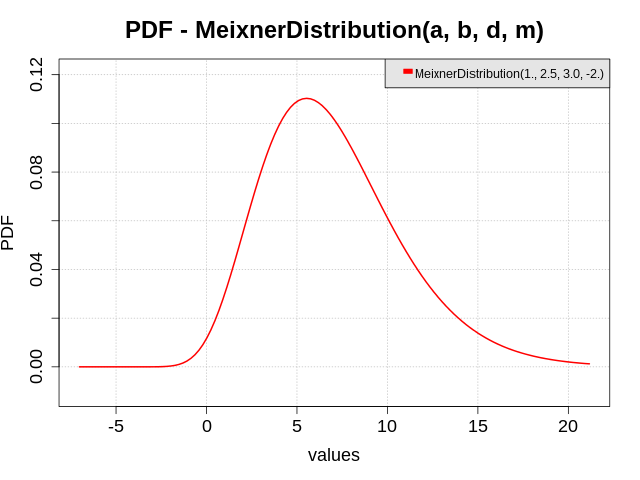
\includegraphics[width=7cm]{Figures/pdf_MeixnerDistribution.png}
\caption{PDF of a  MeixnerDistribution distribution.}
% \label{PDF19}
\end{center}
\end{figure}



\item {\bf Non Central Chi Square}: Univariate distribution. $\vect{\theta} = \left(\nu,\lambda \right)$, with the constraint $\nu>0$ and $\lambda\geq0$. The probability density function writes:
\begin{equation}
f_X(x;\vect{\theta}) = \displaystyle \sum_{j=0}^{\infty} e^{-\lambda}\frac{\lambda^j}{j!}p_{\chi^2(\nu+2j)}(x)
\end{equation}
where $p_{\chi^2(q)}$ is the probability density function of a $\chi^2(q)$ random variate.




\begin{figure}[H]
\begin{minipage}{8cm}
\begin{center}
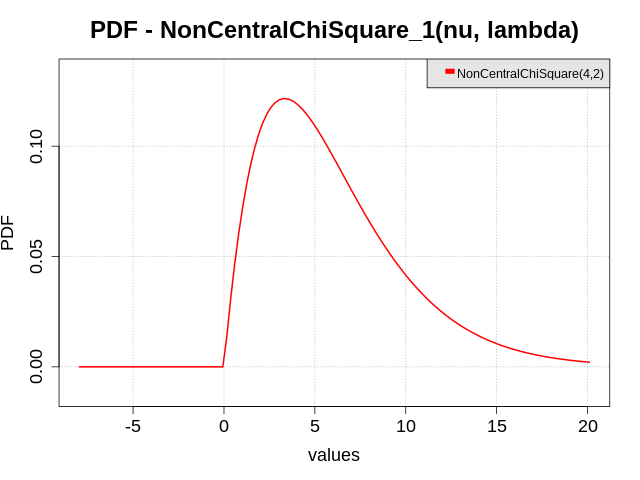
\includegraphics[width=7cm]{Figures/pdf_NonCentralChiSquare_1.png}
\caption{PDF of a Non Central Chi Square distribution.}
% \label{PDF13}
\end{center}
\end{minipage}
\hfill
\begin{minipage}{8cm}
\begin{center}
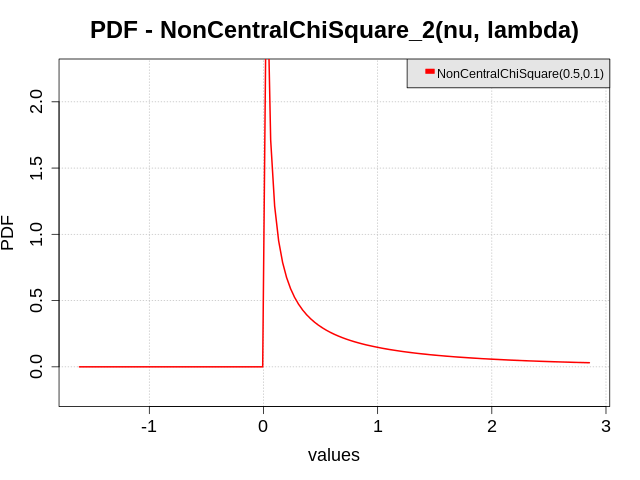
\includegraphics[width=7cm]{Figures/pdf_NonCentralChiSquare_2.png}
\caption{PDF of a  Non Central Chi Square distribution.}
% \label{PDF14}
\end{center}
\end{minipage}
\end{figure}








\item {\bf Non Central Student}: Univariate distribution. $\vect{\theta} = \left(\nu,\delta, \gamma \right)$. Let's note that a random variable $X$ is said to have a standard non-central student distribution $\cT(\nu, \delta)$ if it can be written as:
\begin{equation}
X = \frac{N}{\sqrt{C/\nu}}
\end{equation}
where $N$ has the normal distribution $\cN(\delta, 1)$ and $C$ has the $\chi^2(\nu)$ distribution, $N$ and $C$ being independent.\\
The non-central Student distribution in OpenTURNS has an additional parameter $\gamma$ such that the random variable $X$ is said to have a non-central Student distribution $\cT(\nu, \delta, \gamma)$ if $X-\gamma$ has a standard $\cT(\nu,\delta)$ distribution.\\

We explicitate here the probability density function of the Non Central Student :
\begin{equation}
p_{NCS}(x) = \frac{\exp(-\delta^2 / 2)}{\sqrt{\nu\pi} \Gamma(\nu / 2)}\left(\frac{\nu}{\nu + (x-\gamma)^2}\right) ^ {(\nu + 1) / 2} \sum_{j=0}^{\infty} \frac{\Gamma\left(\frac{\nu + j + 1}{2}\right)}{\Gamma(j + 1)}\left(\delta(x-\gamma)\sqrt{\frac{2}{\nu + (x-\gamma)^2}}\right) ^ j
\end{equation}


\begin{figure}[H]
\begin{center}
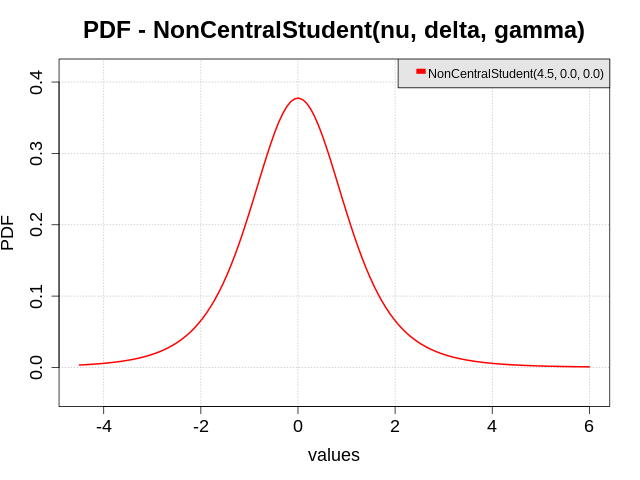
\includegraphics[width=7cm]{Figures/pdf_NonCentralStudent.png}
\end{center}
\caption{PDF of a Non Central Student distribution.}
% \label{PDF19bis}
\end{figure}





\item {\bf Normal Gamma}: Bivariate distribution. $\vect{\theta} = \left(\mu, \kappa, \alpha, \beta \right)$. \\
The Normal Gamma distribution is the distribution of the random vector $(X,Y)$ where $Y$ follows the distribution $\Gamma(\alpha, \beta)$ with $\alpha>0$ and $\beta>0$, $X|Y$ follows the distribution $\mathcal{N}(\mu, \displaystyle \frac{1}{\sqrt{\kappa Y}})$.

We explicitate here the probability density function of the Non Central Student :
\begin{equation}
   p_{NG}(x,y) =  \dfrac{\Gamma(\alpha)}{\beta^\alpha}\sqrt{\dfrac{2\pi}{\kappa}}y^{\alpha-1/2}\exp\left(-\dfrac{y}{2}\left[\kappa(x-\mu)^2+2\beta\right]\right)
\end{equation}




\item {\bf Normal distribution (or Gaussian distribution)}: Multivariate $n$-dimensional distribution. In the case $n=1$, $\vect{\theta} = \left(\mu,\sigma \right)$, with the constraint  $\sigma>0$. The probability density is given as:
\begin{equation}
f_X(x;\vect{\theta}) = \frac{1}{\sigma \sqrt{2\pi}} \exp \left( -\frac{1}{2} \left( \frac{x-\mu}{\sigma} \right)^2 \right)
\end{equation}
The support is $\Rset$. $\mu$ provides the most likely value (for
which the probability density function is at its highest), and the
density function is symmetric around this value (the values
$\mu-a$ and $\mu+a$ are equally likely); $\mu$ is also the
expected value (mean) of this distribution. Whilst $\sigma$
provides a measure of dispersion: the larger it is, the flatter the probability density function is (i.e. values far away from $\mu$ are still likely, or in other words possible values are more spread out).

\begin{figure}[H]
\begin{center}
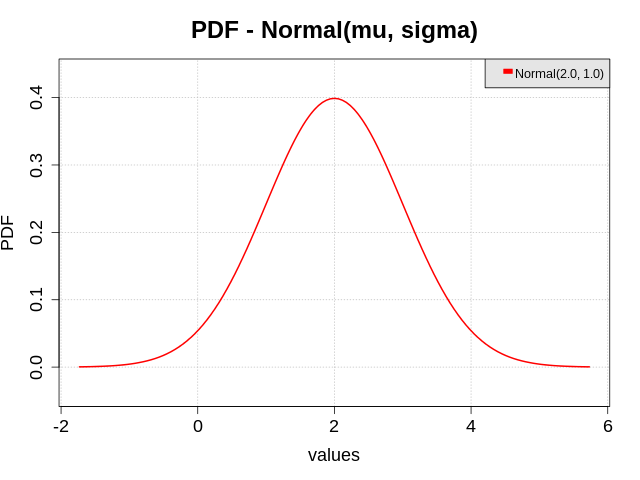
\includegraphics[width=7cm]{Figures/pdf_Normal.png}
\caption{PDF of a Normal distribution.}
% \label{PDF20}
\end{center}
\end{figure}

In dimension $n>1$, the {\bf Multi-Normal Distribution (or Multivariate Normal Distribution)} writes :
\begin{equation}
f_X(x;\vect{\theta}) = \displaystyle
\frac{1}
{
\displaystyle (2\pi)^{\frac{n}{2}}(\mathrm{det}\mat{\Sigma})^{\frac{1}{2}}
}
\displaystyle e^{-\frac{1}{2}\Tr{(\vect{x}-\vect{\mu})}\mat{\Sigma}^{-1^{\strut}}(\vect{x}-\vect{\mu})}
\end{equation}
where  $\mat{\Sigma} = \mat{\Lambda}_{\vect{\sigma}} \mat{R} \mat{\Lambda}_{\vect{\sigma}}$, $\mat{\Lambda}_{\vect{\sigma}} = \mathrm{diag}(\vect{\sigma})$, $\mat{R}$ SPD, $\sigma_i >0$. The distribution is parameterized by  $(\vect{\mu}, \vect{\sigma},\mat{R})$ or $(\vect{\mu}, \mat{\Sigma})$.





\item {\bf Random Mixture distribution}: Univariate distribution. A Random Mixture $Y$ is defined as an affine combination of random variables $X_i$ as follows:
\begin{equation}
\displaystyle Y = a_0 + \sum_{i=1}^n a_i X_i
\end{equation}
where $(a_i)_{ 0 \leq i \leq n} \in \Rset^{n+1}$ and $(X_i)_{ 1 \leq i \leq n}$ are some independent univariate distributions.\\
For example,
\begin{equation}
Y = 2 + 5X_1 + X_2
\end{equation}
where :
\begin{itemize}
\item  $X_1$ follows a $\cE(\lambda = 1.5)$,
\item  $X_3$ follows a $\cN(\mu = 4,Variance = 1)$.
\end{itemize}
The pdf and cdf of this distribution are drawn in Fig.\ref{RMpdf} and Fig.\ref{RMcdf}.


\begin{figure}[H]
\begin{minipage}{8cm}
\begin{center}
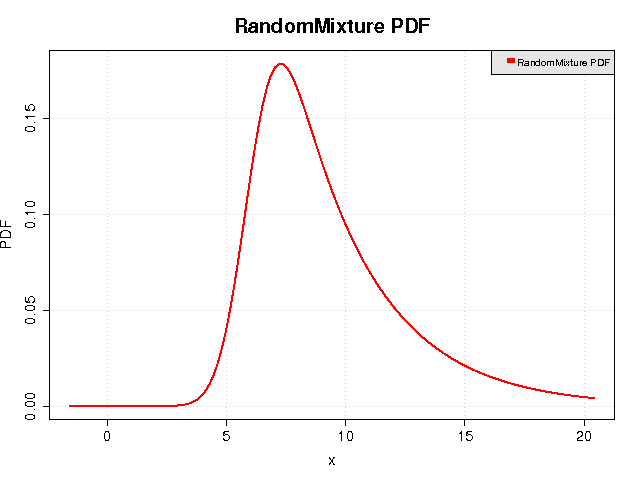
\includegraphics[width=7cm]{Figures/RandomMixture_pdf.png}
\caption{Probability density function of a Random Mixture.}
\label{RMpdf}
\end{center}
\end{minipage}
\hfill
\begin{minipage}{8cm}
\begin{center}
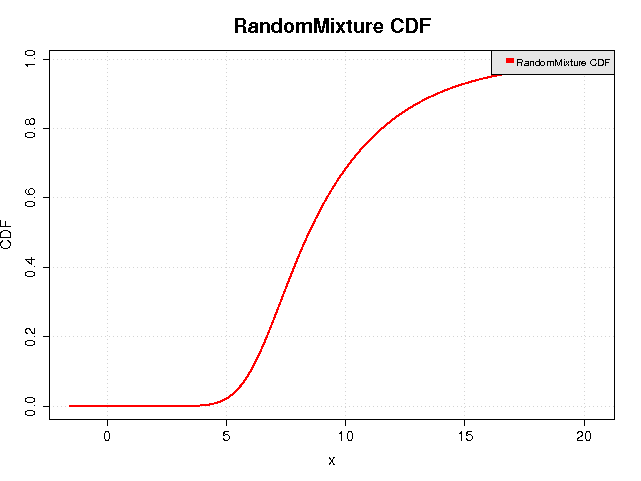
\includegraphics[width=7cm]{Figures/RandomMixture_cdf.png}
\caption{Cumulative density function of a Random Mixture.}
\label{RMcdf}
\end{center}
\end{minipage}
\end{figure}





\item {\bf Rice distribution}:   Univariate distribution. $\vect{\theta} = \left( \sigma, \nu \right)$, with the constraint  $\nu\geq0$ and $\sigma>0$. The probability density is given as:
\begin{equation}
f_X(x;\vect{\theta}) = \displaystyle 2\frac{x}{\sigma^2}p_{\chi^2(2,\frac{\nu^2}{\sigma^2})}(\frac{x^2}{\sigma^2})
\end{equation}
where $p_{\chi^2(\nu, \lambda)}$ is the probability density function of a Non Central Chi Square distribution.



\begin{figure}[H]
\begin{minipage}{8cm}
\begin{center}
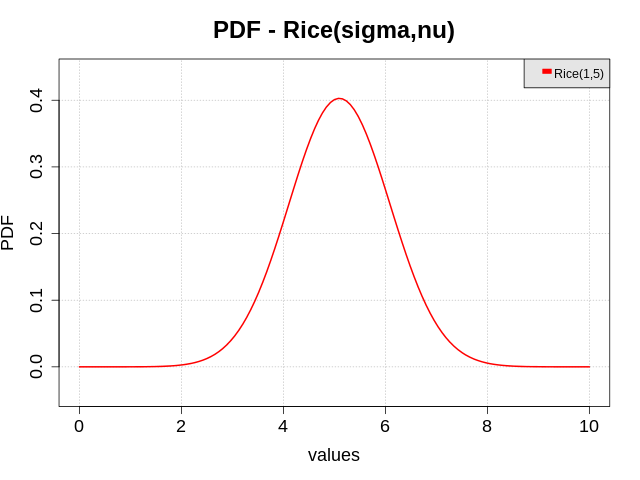
\includegraphics[width=7cm]{Figures/pdf_Rice_1.png}
\caption{Probability density function of a Rice distribution.}
% \label{RMpdf}
\end{center}
\end{minipage}
\hfill
\begin{minipage}{8cm}
\begin{center}
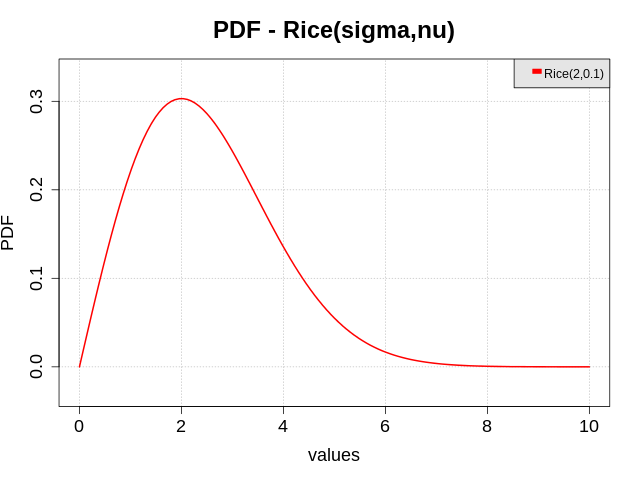
\includegraphics[width=7cm]{Figures/pdf_Rice_2.png}
\caption{Cumulative density function of a Rice distribution.}
% \label{RMcdf}
\end{center}
\end{minipage}
\end{figure}





\item {\bf Rayleigh distribution}:   Univariate distribution. $\vect{\theta} = \left( \sigma, \gamma \right)$, with the constraint  $\sigma>0$.The probability density is given as:
\begin{equation}
f_X(x;\vect{\theta}) = \displaystyle \frac{(x - \gamma)}{\sigma^2}e^{-\frac{(x-\gamma)^2}{2\sigma^2}}\boldsymbol{1}_{[\gamma,+\infty[}(x)
\end{equation}

\begin{figure}[H]
\begin{center}
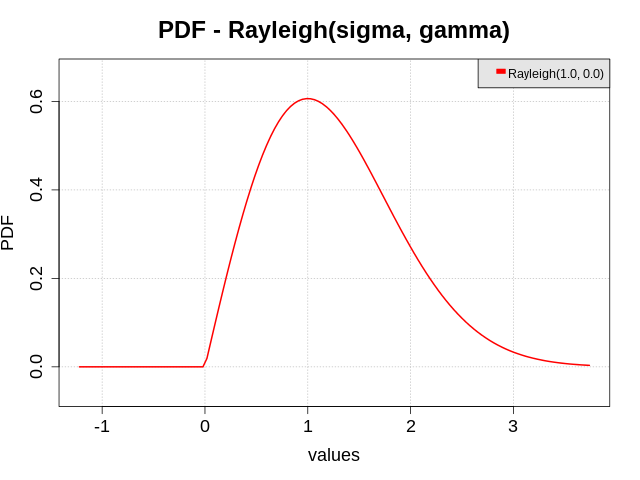
\includegraphics[width=7cm]{Figures/pdf_Rayleigh.png}
\caption{PDF of a Rayleigh distribution.}
% \label{PDF21}
\end{center}
\end{figure}






\item {\bf Student distribution}:  Univariate distribution. $\vect{\theta} = \left( \nu,\vect{\mu}, \vect{\sigma}, \mat{R}\right)$, with the constraint $\nu > 2$.The Student distribution has the following  probability density function, written en dimension $d$ :
\begin{equation}
p_T(\vect{x}) = \frac{\Gamma\left(\frac{\nu+d}{2}\right)}
{(\pi d)^{\frac{d}{2}}\Gamma\left(\frac{\nu}{2}\right)}\frac{\left|\mathrm{det}(\mat{R})\right|^{-1/2}}{\prod_{k=1}^d\sigma_k}\left(1+\frac{\vect{z}^t\mat{R}^{-1}\vect{z}}{\nu}\right)^{-\frac{\nu+d}{2}}
\end{equation}
where $\vect{z}=\mat{\Delta}^{-1}\left(\vect{x}-\vect{\mu}\right)$ with $\mat{\Delta}=\mat{\mathrm{diag}}(\vect{\sigma})$.\\

In dimension $d=1$, $\vect{\theta} = (\nu, \mu, \sigma)$ and the distribution writes :
\begin{equation}
\displaystyle p_T(x) = \frac{\Gamma\left(\frac{\nu+1}{2}\right)}
{\sqrt{\pi}\Gamma\left(\frac{\nu}{2}\right)}\frac{1}{\sigma}\left(1+\frac{(x-\mu)^2}{\nu}\right)^{-\frac{\nu+1}{2}}
\end{equation}
The parameter $\mu$ describes the most likely value. $\nu$ is a measure of dispersion: the probability density function flattens as $\nu$ decreases.

\begin{figure}[H]
\begin{center}
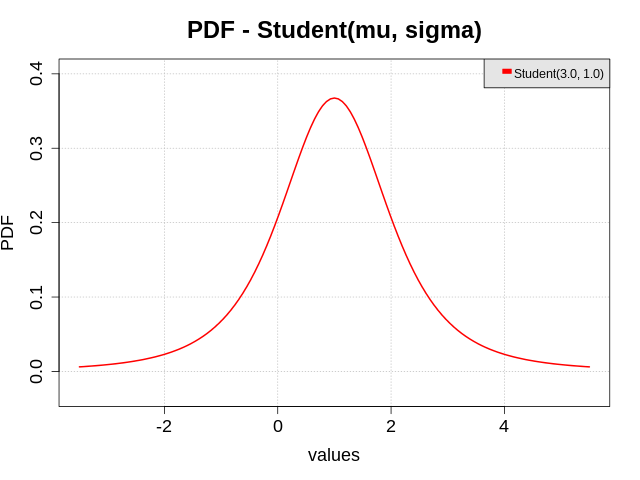
\includegraphics[width=7cm]{Figures/pdf_Student.png}
\caption{PDF of a Student distribution.}
% \label{PDF22}
\end{center}
\end{figure}

\item {\bf Trapezoidal distribution}: $\vect{\theta} = \left(a,b,c,d \right)$, with the constraint $a \leq b < c \leq d$. The probability density function writes:
\begin{equation}
f_X(x;\vect{\theta}) = \left\{
\begin{array}{ll}
\displaystyle h \frac {x-a}{b-a} & \textrm{if}\ a\leq x \leq b \\
\displaystyle h & \textrm{if}\ b\leq x \leq c \\
\displaystyle h \frac{d-x}{d-c}& \textrm{if}\ c\leq x \leq d \\
0 & \textrm{otherwise}
\end{array}
\right.
\end{equation}
with
$h=\frac{2}{d+c-a-b}$\\
The support is $[a,d]$.

\begin{center}
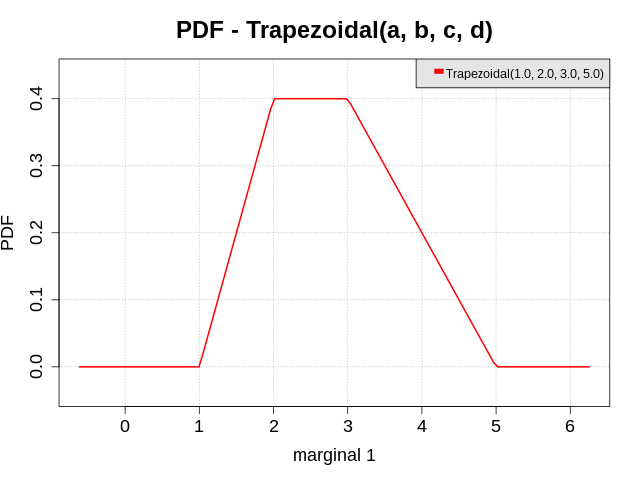
\includegraphics[width=7cm]{Figures/pdf_Trapezoidal.png}
\end{center}


\item {\bf Triangular distribution}: Univariate distribution. $\vect{\theta} = \left(a,b,m \right)$, with the constraints $a \leq m$, $m \leq b$, $b>a$. The probability density function writes:
\begin{equation}
f_X(x;\vect{\theta}) = \left\{
\begin{array}{ll}
\displaystyle 2  \frac{x-a}{(m-a)(b-a)} & \textrm{if}\ a\leq x \leq m \\
\displaystyle 2  \frac{b-x}{(b-m)(b-a)} & \textrm{if}\ m\leq x \leq b \\
0 & \textrm{otherwise}
\end{array}
\right.
\end{equation}
The support is $[a,b]$. $m$ describes the most likely value.

\begin{figure}[H]
\begin{center}
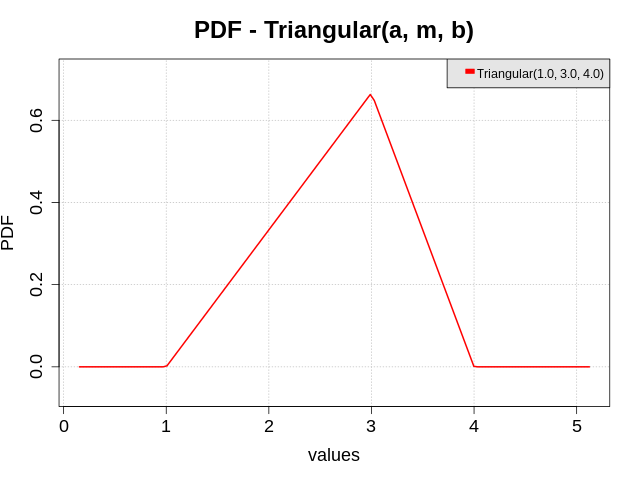
\includegraphics[width=7cm]{Figures/pdf_Triangular.png}
\caption{PDF of a  Triangular distribution.}
% \label{PDF23}
\end{center}
\end{figure}



\item {\bf Truncated Normal Distribution}: Univariate distribution. $\vect{\theta} = \left(\mu_n,\sigma_n,a,b \right)$, with the constraints $\sigma_n>0$, $b>a$. The probability density function writes:
\begin{equation}
f_X(x;\vect{\theta}) = \frac{\varphi(\frac{x-\mu_n}{\sigma_n}) / \sigma_n}{\Phi(\frac{b-\mu_n}{\sigma_n})-\Phi(\frac{a-\mu_n}{\sigma_n})} \mathbf{1}_{a \leq x \leq b}
\end{equation}
where $\varphi$ and $\Phi$ represent the probability density and
the cumulative distribution function respectively of the reduced
centred Normal distribution (i.e. the mean $\mu$ zero and standard
deviation $\sigma$ equal to 1). The support is $[a,b]$. $\mu$ describes the most likely value. Whilst $\sigma$ provides a measure of dispersion: the probability density function flattens as s increases (the probability density becomes zero for values outside the interval $[a,b]$).

\begin{figure}[H]
\begin{minipage}{8cm}
\begin{center}
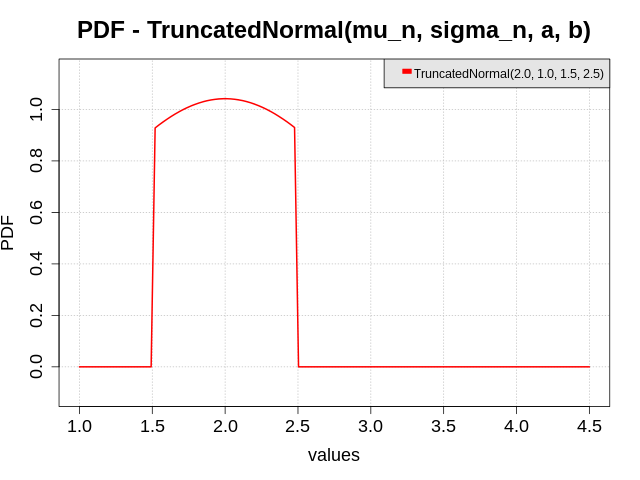
\includegraphics[width=7cm]{Figures/pdf_TruncatedNormal_1.png}
\caption{PDF of a  TruncatedNormal distribution.}
% \label{PDF24}
\end{center}
\end{minipage}
\hfill
\begin{minipage}{8cm}
\begin{center}
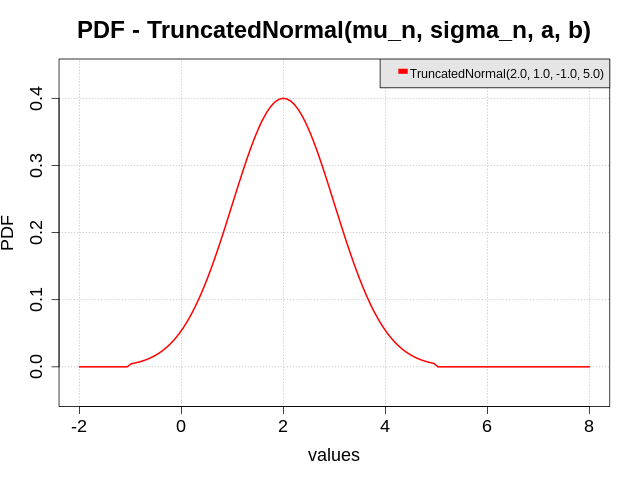
\includegraphics[width=7cm]{Figures/pdf_TruncatedNormal_2.png}
\caption{PDF of a  TruncatedNormal distribution.}
% \label{PDF25}
\end{center}
\end{minipage}
\end{figure}




\item {\bf Uniform distribution}: Univariate distribution.  $\vect{\theta} = \left(a,b \right)$, with the constraint $a < b$. The probability density function writes:
\begin{equation}
f_X(x;\vect{\theta}) = \frac{1}{b-a} \mathbf{1}_{a \leq x \leq b}
\end{equation}
The support is $[a,b]$. All values in this interval are equally-likely.

\begin{figure}[H]
\begin{center}
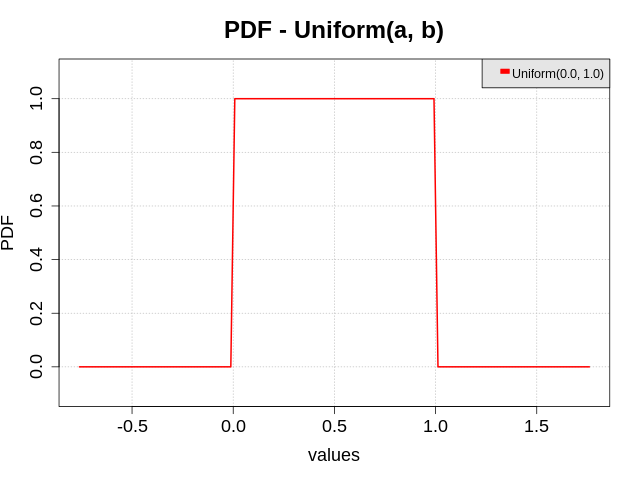
\includegraphics[width=7cm]{Figures/pdf_Uniform.png}
\caption{PDF of a  Uniform distribution.}
% \label{PDF26}
\end{center}
\end{figure}





\item {\bf Weibull distribution}: Univariate distribution. $\vect{\theta} = \left( \alpha,\beta, \gamma \right)$, with the constraints $\alpha>0$, $\beta>0$. probability density function writes:
\begin{equation}
f_X(x;\vect{\theta}) = \frac{\beta}{\alpha} \left( \frac{x-\gamma}{\alpha} \right)^{\beta-1} \exp \left( -\left( \frac{x-\gamma}{\alpha} \right)^\beta \right) \mathbf{1}_{\gamma \leq x}
\end{equation}
The support is $[\gamma,+\infty[$, and is right skewed. Both $\alpha$ and $\beta$ influence the dispersion. We note that the distribution becomes more skewed as $\beta$ decreases. In the case where $\beta = 1$ this is corresponds to the Exponential distribution.

\begin{figure}[H]
\begin{minipage}{8cm}
\begin{center}
\includegraphics[width=7cm]{Figures/pdf_Weibull_1.png}
\caption{PDF of a  Weibull distribution.}
% \label{PDF27}
\end{center}
\end{minipage}
\hfill
\begin{minipage}{8cm}
\begin{center}
\includegraphics[width=7cm]{Figures/pdf_Weibull_2.png}
\caption{PDF of a Weibull distribution.}
% \label{PDF28}
\end{center}
\end{minipage}
\end{figure}


\item {\bf Wishart distribution}: Multivariate distribution. $\vect{\theta} = \left( \mat{V},\nu \right)$ where $\mat{V}$ is a symmetric positive definite matrix of dimension $p$ and $\nu>p-1$. The probability density function writes:
\begin{equation}
f_{\vect{x}}(\vect{x};\vect{\theta}) = \frac{|m(\vect{x})|^{\frac{\nu-p-1}{2}}e^{-\frac{\mathrm{tr}(\mat{V}^{-1}m(\vect{x}))^{\strut}}{2}}}{2^{\frac{\nu p}{2}}|\mat{V}|^{\frac{\nu}{2}}\Gamma_p\left(\frac{\nu}{2}\right)_{\strut}}\fcar{\cM_p^+(\Rset)}{m(\vect{x})}
\end{equation}
where $\vect{x}\in\Rset^{\frac{p(p+1)}{2}}$, $\cM_p^+(\Rset)$ is the set of symmetric positive matrices of dimension $p$ and $m:\Rset^{\frac{p(p+1)}{2}}\rightarrow\cM_p^+(\Rset)$ is given by:
\begin{align}
  m(\vect{x})=\left(\begin{array}{cccc}
x_1 & x_2 & \cdots &  x_{1+p(p-1)/2}\\
x_2 & x_3 &  & \vdots \\
\vdots & & \ddots & \vdots\\
x_{1+p(p-1)/2} & \cdots & \cdots & x_{p(p+1)/2}
\end{array}
\right)
\end{align}


\end{itemize}



OpenTURNS also proposes some Discrete Distributions.

\begin{itemize}

\item {\bf Bernoulli distribution}: Univariate distribution. $\vect{\theta} = p$, with the constraint $0<p<1$. The Bernoulli distribution takes only 2 values : 0 and 1.
\begin{equation}
\Prob{X = 1} = p, \, \Prob{X = 0} = 1-p
\end{equation}

\begin{figure}[H]
\begin{minipage}{8cm}
\begin{center}
\includegraphics[width=7cm]{Figures/pdf_Bernoulli.png}
\caption{Distribution of a Bernoulli distribution.}
\label{PDFBernoulli}
\end{center}
\end{minipage}
\hfill
\begin{minipage}{8cm}
\begin{center}
\includegraphics[width=7cm]{Figures/cdf_Bernoulli.png}
\caption{CDF of a Bernoulli distribution.}
\label{CDFBernoulli}
\end{center}
\end{minipage}
\end{figure}

\item {\bf Binomial distribution}: Univariate distribution. $\vect{\theta} = (n,p)$, with the constraint $0<p<1$ and . The Binomial distribution values are the integer between 0 and n.
\begin{equation}
\displaystyle P(X = k) = C_n^k p^k (1-p)^{{n-k}}
\end{equation}
where
\begin{equation}
\begin{array}{@{}l@{}}
k^{\strut} \in \{0, \hdots, n\} \\
n \in \Nset \\
p \in [0,1]
\end{array}
\end{equation}



\begin{figure}[H]
\begin{minipage}{8cm}
\begin{center}
\includegraphics[width=7cm]{Figures/pdf_Binomial.png}
\caption{Distribution of a Binomial distribution.}
\label{PDFBinomial}
\end{center}
\end{minipage}
\hfill
\begin{minipage}{8cm}
\begin{center}
\includegraphics[width=7cm]{Figures/cdf_Binomial.png}
\caption{CDF of a Binomial distribution.}
\label{CDFBinomial}
\end{center}
\end{minipage}
\end{figure}


\item {\bf Dirac distribution}: Multivariate distribution. $\vect{\theta} = point$. The Dirac distribution takes only one value : $point\in\Rset^n$.
\begin{equation}
\Prob{\vect{X} = point} = 1
\end{equation}

\begin{figure}[H]
\begin{minipage}{8cm}
\begin{center}
\includegraphics[width=7cm]{Figures/pdf_Dirac.png}
\caption{Distribution of a Dirac distribution.}
\label{PDFDirac}
\end{center}
\end{minipage}
\hfill
\begin{minipage}{8cm}
\begin{center}
\includegraphics[width=7cm]{Figures/cdf_Dirac.png}
\caption{CDF of a Dirac distribution.}
\label{CDFDirac}
\end{center}
\end{minipage}
\end{figure}




\item {\bf Geometric distribution}: Univariate distribution. $\vect{\theta} = p$, with the constraint $0<p<1$. all natural numbers $k \in \Nset^*$,
\begin{equation}
\Prob{X = k ; \vect{\theta}} = p \left(1-p\right)^{k-1}
\end{equation}
The support is $\Nset^*$.

\begin{figure}[H]
\begin{minipage}{8cm}
\begin{center}
\includegraphics[width=7cm]{Figures/pdf_Geometric.png}
\caption{Distribution of a Geometric distribution.}
\label{PDFGeometric}
\end{center}
\end{minipage}
\hfill
\begin{minipage}{8cm}
\begin{center}
\includegraphics[width=7cm]{Figures/cdf_Geometric.png}
\caption{CDF of a Geometric distribution.}
\label{CDFGeometric}
\end{center}
\end{minipage}
\end{figure}



\item {\bf KPermutationsDistribution distribution}: Multivariate
$d$-dimensional distribution. $\vect{\theta} = ( k,n)$, with the
constraints $n \geq 1$ and $k \geq 1$. The
\textit{KPermutationsDistribution} is the discrete uniform distribution
on the set of injective functions $(i_0, \hdots, i_{k_1})$ from $\{0, \dots, k-1\}$ into
$\{0, \dots, n-1\}$:
\begin{equation}
\displaystyle P(\vect{X} = (i_0, \hdots, i_{k-1})) = \frac{1}{d}
\end{equation}
where $d=A_n^k=\displaystyle \frac{n!}{(n-k)!}$.


\item {\bf Multinomial distribution}: Multivariate $n$-dimensional distribution. $\vect{\theta} = ((p_k)_{1 \leq k \leq n}, N)$, with the constraint $0<p<1$ and $x_i \in \Nset^*$,
\begin{equation}
\displaystyle P(\vect{X} = \vect{x}) = \frac{N!}{x_1!\dots x_n! (N-s)!}p_1^{x_1}\dots p_n^{x_n}(1-q)^{N-s}
\end{equation}
where
\begin{equation}
\begin{array}{@{}l@{}}
0^{\strut}\leq p_i \leq 1 \\
x_i\in \Nset \\
\displaystyle q = \sum_{k=1}^n p_k \leq 1 \\
s=  \sum_{k=1}^n x_k \leq N_{\strut}
\end{array}
\end{equation}
In dimension $n=1$, this definition corresponds to the Binomial distribution.



\item {\bf Negative Binomial distribution}: Univariate distribution. $\vect{\theta} = (r,p)$, with the constraint $0<p<1$ and $r>0$. The Negative Binomial distribution values are the positive integers $0,1,\dots$
\begin{equation}
\displaystyle P(X = k) = \frac{\Gamma(k + r)}{\Gamma(r)\Gamma(k+1)}p^k(1-p)^r
\end{equation}
where $k\in\Nset$

\begin{figure}[H]
\begin{minipage}{8cm}
\begin{center}
\includegraphics[width=7cm]{Figures/pdf_NegativeBinomial.png}
\caption{Distribution of a Negative Binomial distribution.}
\label{PDFNegativeBinomial}
\end{center}
\end{minipage}
\hfill
\begin{minipage}{8cm}
\begin{center}
\includegraphics[width=7cm]{Figures/cdf_NegativeBinomial.png}
\caption{CDF of a Negative Binomial distribution.}
\label{CDFNegativeBinomial}
\end{center}
\end{minipage}
\end{figure}



\item {\bf Poisson distribution}: Univariate distribution. $\vect{\theta} = \lambda$, with the constraint $\lambda > 0$. For all $k \in \Nset$,
\begin{equation}
\Prob{X = k ; \vect{\theta}} = \frac{\lambda^k}{k!} \exp \left( -\lambda \right)
\end{equation}

The support is $\Nset$.


\begin{figure}[H]
\begin{minipage}{8cm}
\begin{center}
\includegraphics[width=7cm]{Figures/pdf_Poisson.png}
\caption{Distribution of a Poisson distribution.}
\label{PDFPoisson}
\end{center}
\end{minipage}
\hfill
\begin{minipage}{8cm}
\begin{center}
\includegraphics[width=7cm]{Figures/cdf_Poisson.png}
\caption{CDF of a Poisson distribution.}
\label{CDFPoisson}
\end{center}
\end{minipage}
\end{figure}


\item {\bf Skellam distribution}: Univariate distribution. $\vect{\theta} = (\lambda_1, \lambda_2)$, with the constraint $\lambda_i>0$. The Skellan distribution takes its values in $\Zset$. It is the distribution of $(X_1-X_2)$ for $(X_1, X_2)$ independant and respectively distributed according to $Poisson(\lambda_i)$. The probability distribution function is:
\begin{equation}
\forall k \in \Zset, \quad \Prob{X = k} = 2\Prob{Y=2\lambda_1}
\end{equation}
where $Y$ is distributed according to the  the non central chi-square distribution $\chi^2_{\nu, \delta}$, with $\nu=2(k+1)$ and $\delta=2\lambda_2$.



\begin{figure}[H]
\begin{minipage}{8cm}
\begin{center}
\includegraphics[width=7cm]{Figures/pdf_Skellam.png}
\caption{Distribution of a  Skellam distribution.}
\label{PDFSkellam}
\end{center}
\end{minipage}
\hfill
\begin{minipage}{8cm}
\begin{center}
\includegraphics[width=7cm]{Figures/cdf_Skellam.png}
\caption{CDF of a Skellam distribution.}
\label{CDFSkellam}
\end{center}
\end{minipage}
\end{figure}




\item {\bf UserDefined}:  Multivariate $n$-dimensional distribution. $\vect{\theta} = (\vect{x_k}, p_k)_{1 \leq k \leq N}$, with the constraint $\lambda > 0$, where $0\leq p_k \leq 1$, $\displaystyle \sum_{k=1}^{N^{\strut}} p_k = 1$.
\begin{equation}
P(\vect{X} = \vect{x}_k) = p_k)_{1 \leq k \leq N}
\end{equation}

The support is $\Nset$.


\begin{figure}[H]
\begin{minipage}{8cm}
\begin{center}
\includegraphics[width=7cm]{Figures/pdf_UserDefined.png}
\caption{Distribution of a  UserDefined distribution.}
\label{PDFUserDefined}
\end{center}
\end{minipage}
\hfill
\begin{minipage}{8cm}
\begin{center}
\includegraphics[width=7cm]{Figures/cdf_UserDefined.png}
\caption{CDF of a UserDefined distribution.}
\label{CDFUserDefined}
\end{center}
\end{minipage}
\end{figure}



\item {\bf Zipf-Mandelbrot distribution}: Univariate distribution. $\vect{\theta} = \left( N,q,s \right)$, with the constraints $N \geq 1$, $q \geq 0$ and $s>0$. For all $k \in [1,N]$, $k$ integer,
\begin{equation}
\forall k\in [1,N], P(X=k) = \frac{1}{(k+q)^s} \frac{1}{H(N,q,s)}
\end{equation}
where $H(N,q,s)$ is the Generalized Harmonic Number : $H(N,q,s) = \sum_{i=1}^{N} \displaystyle \frac{1}{(i+q)^s}$.

\begin{figure}[H]
\begin{minipage}{8cm}
\begin{center}
\includegraphics[width=7cm]{Figures/pdf_ZipfMandelbrot_1.png}
\caption{Distribution of a  Zipf-Mandelbrot distribution.}
\label{PDFZipfMandelbrot}
\end{center}
\end{minipage}
\hfill
\begin{minipage}{8cm}
\begin{center}
\includegraphics[width=7cm]{Figures/cdf_ZipfMandelbrot_1.png}
\caption{CDF of a Zipf-Mandelbrot  distribution.}
\label{CDFZipfMandelbrot}
\end{center}
\end{minipage}
\end{figure}

\end{itemize}


\underline{\textbf{Standard representative of distributions}} \vspace{2mm}


OpenTURNS associates to each distribution a standard representative, corresponding to a specific set of its parameters. The following tabulars detail the specific set of parameters and gives the expression of its non centered moments of order $n$.

% \begin{itemize}
% \item Continous distributions :
% \end{itemize}

% \begin{table}[H]
%   \begin{center}
%     \noindent \begin{tabular}{|c|c|}
%       \hline
%       Standard representative parameters & Raw moment of order $N$ \\
%       \hline
%       \hline
%       \multicolumn{2}{|c|}{ArcSine} \\
%       \hline
%       & & \\
%       \hline
%       \multicolumn{2}{|c|}{Beta} \\
%       \hline
%       & & \\
%       \hline
%       \multicolumn{2}{|c|}{Burr} \\
%       \hline
%       & & \\
%       \hline
%       \multicolumn{2}{|c|}{Chi} \\
%       \hline
%       & & \\
%       \hline
%       \multicolumn{2}{|c|}{ChiSquare} \\
%       \hline
%       & & \\
%       \hline
%       \multicolumn{2}{|c|}{Dirichlet} \\
%       \hline
%       & & \\
%       \hline
%       \multicolumn{2}{|c|}{Epanechnikov} \\
%       \hline
%       & & \\
%       \hline
%       \multicolumn{2}{|c|}{Exponential} \\
%       \hline
%       & & \\
%       \hline
%       \multicolumn{2}{|c|}{Fisher-Snedecor} \\
%       \hline
%       & & \\
%       \hline
%       \multicolumn{2}{|c|}{Gamma} \\
%       \hline
%       & & \\
%       \hline
%       \multicolumn{2}{|c|}{Gumbel} \\
%       \hline
%       & & \\
%       \hline
%       \multicolumn{2}{|c|}{Histogram} \\
%       \hline
%       & & \\
%       \hline
%       \multicolumn{2}{|c|}{Inverse Normal} \\
%       \hline
%       & & \\
%       \hline
%       \multicolumn{2}{|c|}{Laplace} \\
%       \hline
%       & & \\
%       \hline
%       \multicolumn{2}{|c|}{Logistic} \\
%       \hline
%       & & \\
%       \ifpdf % Manual splitting of the tabular in PDF mode
%     \end{tabular}
%   \end{center}
% \end{table}

% \begin{table}[H]
%   \begin{center}
%     \noindent \begin{tabular}{|c|c|}
%       \hline    %
%       Standard representative parameters & Raw moment of order $N$ \\
%       \hline
%       \fi % Manual splitting of the tabular in PDF mode
%       \multicolumn{2}{|c|}{LogNormal} \\
%       \hline
%       & & \\
%       \hline
%       \multicolumn{2}{|c|}{LogUniform} \\
%       \hline
%       & & \\
%       \hline
%       \multicolumn{2}{|c|}{Non Central Chi Square} \\
%       \hline
%       & & \\
%       \hline
%       \multicolumn{2}{|c|}{Non Central Student} \\
%       \hline
%       & & \\
%       \hline
%       \multicolumn{2}{|c|}{Normal (1d)} \\
%       \hline
%       & & \\
%       \hline
%       \multicolumn{2}{|c|}{Rayleigh} \\
%       \hline
%       & & \\
%       \hline
%       \multicolumn{2}{|c|}{Rice} \\
%       \hline
%       & & \\
%       \hline
%       \multicolumn{2}{|c|}{Student (1D)} \\
%       \hline
%       & & \\
%       \hline
%       \multicolumn{2}{|c|}{Trapezoidal} \\
%       \hline
%       & & \\
%       \hline
%       \multicolumn{2}{|c|}{Triangular} \\
%       \hline
%       %       $\left(-1, \mu, 1\right)$ with $\mu=\dfrac{2m-a-b}{b-a}$ & $\begin{array}{rl}
%       %         2\dfrac{1 - \mu^{N+2}}{(N + 1)(N + 2)(1 - \mu^2)}&\mbox{for even }N\\
%       %         2\mu\dfrac{1 - \mu^{N+1}}{(N + 1)(N + 2)(1 - \mu^2)}&\mbox{for odd }N
%       %       \end{array}$\\
%       \hline
%       \multicolumn{2}{|c|}{Truncated Normal} \\
%       \hline
%       %       $\left(2\mu-\dfrac{a+b}{b-a},\dfrac{2\sigma}{b-a},-1,1\right)$ & $\int_{-1}^1x^Np(x)\,\Diff x$\\
%       \hline
%       \multicolumn{2}{|c|}{Uniform} \\
%       \hline
%       %       $(-1,1)$ & $\dfrac{1}{N+1}$ \\
%       \hline
%       \multicolumn{2}{|c|}{Weibull} \\
%       \hline
%       %       $(1, \beta, 0)$ & $\Gamma\left(1+\dfrac{N}{\beta}\right)$ \\
%       \hline
%     \end{tabular}
%   \end{center}
% \end{table}


% \begin{itemize}
% \item Discrete distributions :
% \end{itemize}

% \begin{table}[H]
%   \begin{center}
%     \noindent \begin{tabular}{|c|c|c|}
%       \hline    %
%       Name & Standard representative parameters & Raw moment of order $N$ \\
%       \hline

%       Bernoulli & & \\
%       \hline
%       Binomial & & \\
%       \hline
%       Dirac & & \\
%       \hline
%       Geometric & & \\
%       \hline
%       Multinomial (nD) & & \\
%       \hline
%       Negative Binomial & & \\
%       \hline
%       Poisson & & \\
%       \hline
%       User defined (nD) & $(\vect{x}_k, w_k)_{k=0,\hdots,n-1}$ & $\sum_{k=0}^{n-1} \vect{x}_i^Np(\vect{x}_k)$ \\
%       \hline
%       Zipf-Mandelbrot & $(n, q, s)$ & $\sum_{k=0}^n k^Np(k)$\\
%       \hline
%     \end{tabular}
%   \end{center}
% \end{table}
}
{
-
}

\Methodology{
These probability distributions can be used in step B "Quantifying Sources of Uncertainty". Choosing a probability distribution is equivalent to implicitly making a hypothesis on the type of uncertainty of one of the variables $\vect{X}$ defined in step A "Specifying Criteria and the Case Study".
}
{
This parametric approach has the advantage to feature the uncertainty using a reduced number of parameters. This is particularly useful when there is little data available for the unknown variables (situation in which a non-parametric approach would be limited -- see \otref{docref_B11_EmpiricalCDF}{empirical distribution function} and \otref{docref_B11_KernelSmoothing}{kernel smoothing}) and even when there is no data (the analysis can thus only rely on expert judgement, easier to interpret when there are few distribution parameters). \vspace{2mm}

Moreover, a parametric approach is often preferable when the uncertainty study criterion defined in step A deals with a rare event, obtaining a precise evaluation of the necessary criteria generally necessitates the extrapolation of X values from the observed data. Beware however! An unwise modelling assumption (bad choice of distribution) can lead to an erroneous extrapolation and thus the results of the study may be false! \vspace{2mm}

The correct choice of probability distribution is thus crucial. Statistical tools are available to validate or invalidate the choice of distribution given a set of data (see for example \otref{docref_B221_Graph}{Graphical analysis} \otref{docref_B222_TestKS}{Kolmogorov-Smirnov test}). But consideration of the underlying context is also recommended. For example:
\begin{itemize}
\item    the Normal distribution is relevant in metrology to represent certain measures of uncertainty.
\item    the Exponential distribution is useful for modelling uncertainty when considering the life duration of material that is not subject to ageing,
\item    the Gumbel distribution is defined to describe extreme phenomenon (e.g. maximal annual flow of a river or of wind speed)
\end{itemize}
\vspace{2mm}

Some distributions are often used to express expert judgement in simple terms:
\begin{itemize}
\item the Uniform distribution expresses knowledge concerning the absolute limits of variables (i.e. the probability to exceed these limits is strictly zero) without any other prior assumption about the distribution (such as, for example the mean value or the most likely value),
\item the Triangular distribution expresses knowledge concerning the absolute limits of variables and the most likely value.
\end{itemize}

Finally, an important point concerning the multi-dimensional case where $n_X > 1$. Choosing the type of distribution implies an assumption about the uncertainty of each of the variables $X^i$, but also on the potential inter-dependencies between variables. These inter-dependencies between unknown variables can consequently have an impact on the results of the uncertainty study.

Readers wishing to consider the dependencies in their study more deeply are referred to, for example, \otref{docref_B122_Copulas}{copula method}, \otref{docref_B231_Pearson}{linear correlation}, \otref{docref_B232_Spearman}{rank correlation}. \vspace{2mm}

The following bibliographical references provide main starting points for further study of this method:
\begin{itemize}
\item Saporta, G. (1990). "Probabilités, Analyse de données et Statistique", Technip
\item Dixon, W.J. \& Massey, F.J. (1983) "Introduction to statistical analysis (4th ed.)", McGraw-Hill
\item Bhattacharyya, G.K., and R.A. Johnson, (1997). "Statistical Concepts and Methods", John Wiley and Sons, New York.
\end{itemize}
}
